\documentclass[11pt,a4paper]{article}
\usepackage[hyperref]{acl}
\usepackage{times}
\usepackage{latexsym}
\usepackage{microtype}
\usepackage{graphicx}
\usepackage{booktabs}
\usepackage{multirow}
\usepackage{amsmath,amssymb}
\usepackage{url}
\def\UrlBreaks{\do\/\do\-\do\.\do\_}
\usepackage{tabularx}
\usepackage{adjustbox}
\usepackage{subcaption}
\usepackage{xcolor}

\usepackage{tikz}
\usetikzlibrary{arrows.meta,positioning,shapes.geometric,fit,calc}

% Float placement parameters for compact 6-page layout
\setcounter{topnumber}{3}
\setcounter{bottomnumber}{2}
\setcounter{totalnumber}{4}
\setcounter{dbltopnumber}{1}
\renewcommand{\topfraction}{0.95}
\renewcommand{\bottomfraction}{0.85}
\renewcommand{\dbltopfraction}{0.95}
\renewcommand{\textfraction}{0.05}
\renewcommand{\floatpagefraction}{0.8}
\renewcommand{\dblfloatpagefraction}{0.8}
\setlength{\floatsep}{5pt plus 1pt minus 1pt}
\setlength{\textfloatsep}{7pt plus 1pt minus 2pt}
\setlength{\intextsep}{5pt plus 1pt minus 1pt}
\setlength{\dbltextfloatsep}{7pt plus 1pt minus 2pt}
\setlength{\abovecaptionskip}{3.5pt}
\setlength{\belowcaptionskip}{1.5pt}
% Fallback box for screenshots still pending capture (used with \IfFileExists).
\newcommand{\screenshotplaceholder}[4]{%
  \fbox{\parbox[c][#2][c]{\dimexpr#1-2\fboxsep-2\fboxrule\relax}{\centering\footnotesize\textbf{#3}\\[0.3em]#4}}%
}

% Define a clean, robust placeholder figure box for exact dimensioning
\newcommand{\placeholderbox}[4]{%
  \fbox{%
    \begin{minipage}[c][#2][c]{\dimexpr#1-2\fboxsep-2\fboxrule\relax}%
      \centering\sffamily%
      {\bfseries #3}\par\vspace{0.4em}%
      {\footnotesize\color{black!75} #4}%
    \end{minipage}%
  }%
}

\title{KrishokTech: Deterministic-First, Evidence-Bounded Bengali Agricultural Advisory}

\author{
  Khan Raiyan Ibne Reza \quad Sanjana Aktar Maria \quad Shakil Ahmed \quad Sumaiya Tabassum Nimi \\
  Department of Computer Science and Engineering \\
  North South University, Dhaka 1229, Bangladesh \\
  \texttt{\{raiyan.reza, sanjana.maria, shakil.ahmed02, sumaiya.nimi\}@northsouth.edu}
}

\date{}

\raggedbottom
\begin{document}
\maketitle

\begin{abstract}
A farmer who asks which pesticide to spray, without naming the crop, should get a question back before any answer. \textsc{KrishokTech} is a Bengali agricultural advisory system that keeps such decisions away from the language model. Before generation, rule-based checks refer policy-covered high-risk requests to a helpline, halt treatment requests that name no crop, scope retrieval to one crop, and ask the farmer to confirm when a photograph and the text name different crops. After generation, a verifier withholds dosage claims that the retrieved BARI/BRRI evidence does not support. The demonstration shows each decision as ASK, CONFIRM, REFER, or DROP, together with the sources behind it. On 200 real farmer queries, the gate halted all 30 crop-less requests before retrieval and passed the other 170. Binding the crop lowered top-five cross-crop retrieval from 36.25\% to 30.0\% on 400 stress queries. The mismatch check caught 53 of 54 farmer conflicts and all 400 synthetic ones without halting any matched control, and the dosage verifier caught 114 of 118 inserted errors while accepting all 38 original answers.
\end{abstract}

% =========================================================================
% SECTION 1: INTRODUCTION
% =========================================================================
\section{Introduction}
\label{sec:introduction}

\begin{figure*}[t]
\centering
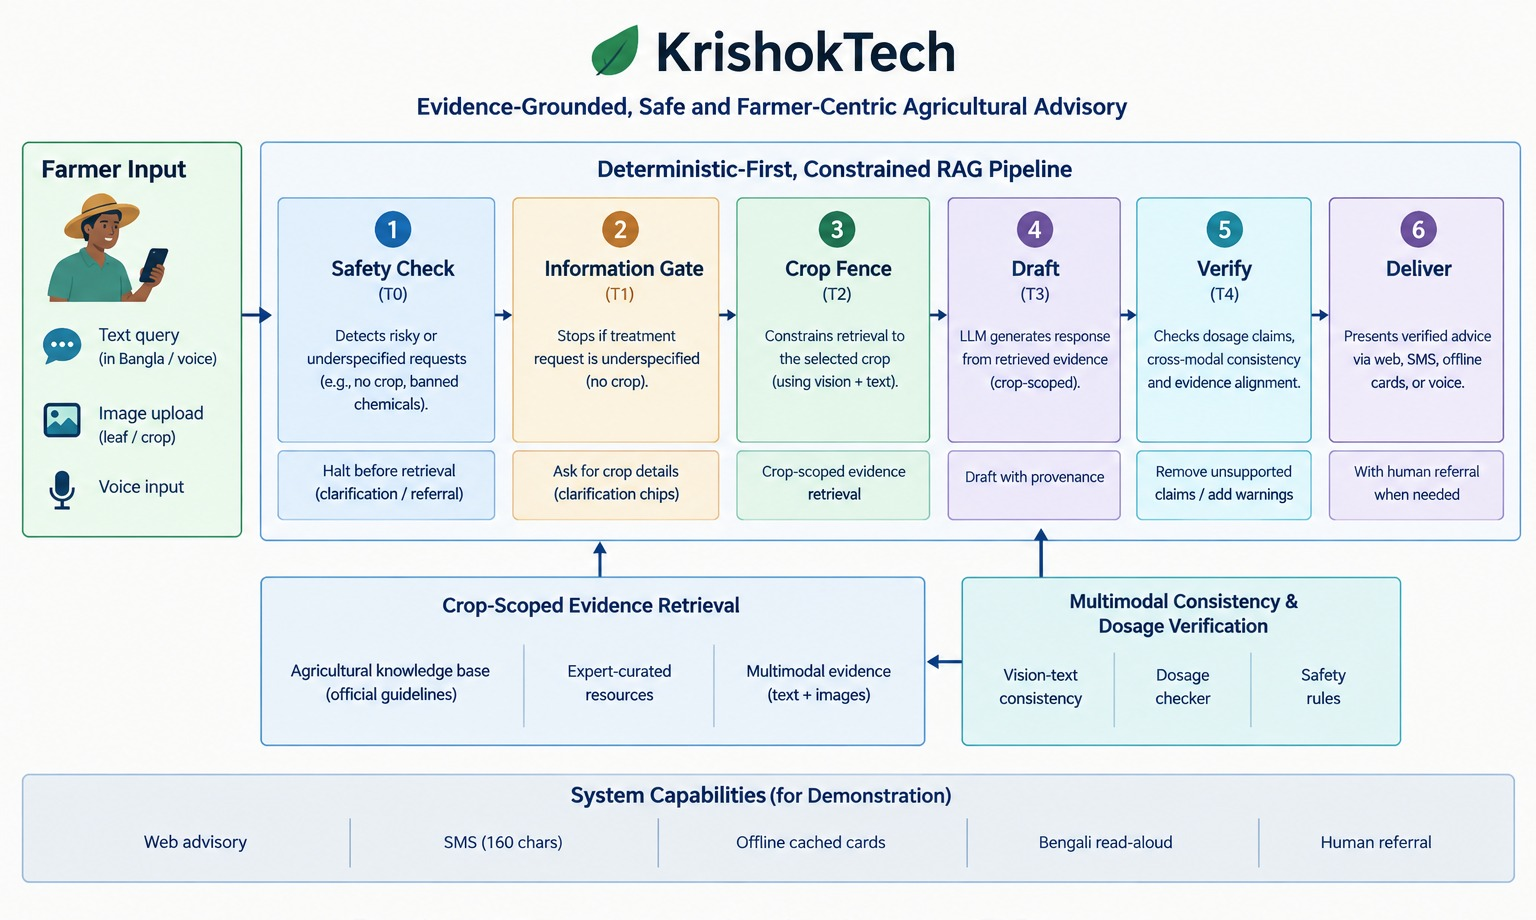
\includegraphics[width=\textwidth]{figures/fig1_architecture.jpg}
\caption{KrishokTech uses five control stages (T0--T4), followed by delivery. T0 can end a request in \textbf{REFER}, T1 in \textbf{ASK}, and T2 in \textbf{CONFIRM}. T3 produces an unverified draft; T4 \textbf{DROP}s unsupported dosage claims from it before the rest is delivered.}
\label{fig:architecture}
\end{figure*}

When yellow spots appear on potato leaves, a farmer often needs advice before an extension officer can visit. Digital advisory services can narrow this gap \citep{dae_extension_manual,aker-2011-dial-a,fabregas-etal-2019-digital}, but treatment advice is safety-critical: an answer for the wrong crop or an unsupported dosage can turn an incomplete question into a harmful recommendation.

A farmer may ask ``which pesticide should I spray?'' without naming the crop. The problem therefore starts before generation: retrieval may search unrelated guidance, and a plausible dosage may be drawn from the wrong evidence. Farmer queries often use colloquial or Romanized Bangla, which differs from the formal terminology of agricultural manuals \citep{bhuiyan-etal-2025-bhasabodh,our_bengali_retrieval,parikh-solorio-2021-normalization}. Photographs and text can disagree, and silently choosing one leaves the conflict unresolved \citep{Deng_2025_CVPR,zhu2024cross}. Even with relevant evidence, generated claims may drift from their context \citep{brown-etal-2025-rag,xu-etal-2025-mega-rag}, and a wrong numerical dose is directly actionable \citep{our_agricultural_safety}.

\textsc{KrishokTech} is built for farmers and the extension officers who support them. It separates drafting an answer from deciding whether that answer may proceed. The model writes drafts; three rule-based controls decide the rest, and each outcome is shown to the farmer as a named state (Figure~\ref{fig:architecture}): (\textbf{C1}) \emph{admission}: policy-covered high-risk requests end in \textbf{REFER}, and treatment requests without a crop end in \textbf{ASK} before retrieval; (\textbf{C2}) \emph{evidence binding}: retrieval is scoped to one crop, and a text--image crop conflict ends in \textbf{CONFIRM} until the farmer resolves it; (\textbf{C3}) \emph{release}: dosage claims that the retrieved passages and BARI/BRRI dose ranges do not support are \textbf{DROP}ped before rendering.

Two further properties support these controls. First, Bengali and Banglish normalization runs before C1 and C2, so colloquial and Latin-script spellings reach the same checks as formal text. Second, agricultural knowledge lives in an external evidence index rather than in model weights. A general-purpose model cannot be assumed to know which chemicals and dose ranges current BARI, BRRI, and DAE guidance permits for each crop, whereas curated passages can be revised without retraining the generator. This also allows a small local generator for offline and privacy-sensitive use.

Our contribution is this integrated, inspectable workflow: an ordered set of admission, evidence, and release controls around a replaceable generator, with each decision visible in the interface and traceable to its source. We report measured behavior of each control on bounded test sets. We do not claim that dialect understanding is solved or that the system improves outcomes in the field.

The demonstration follows a farmer through these states, from a colloquial crop-less query to crop-scoped evidence, a text--image conflict, a safety referral, and an answer whose dosage has been checked (Section~\ref{sec:demonstration}). Interactive demo: \url{https://krishoktech-one.vercel.app}; screencast (\textless{}2.5\,min): \url{https://krishoktech-one.vercel.app/screencast}. Code: \url{https://github.com/RaiyaanReza/KrishokChat-Agricultural-Advisory-System}.

% =========================================================================
% SECTION 2: RELATED WORK AND POSITIONING
% =========================================================================
\section{Related Work and Positioning}
\label{sec:related_work}

Digital agricultural advisors such as Farmer.Chat, KrishokBondhu, and Krishi Sathi pair localized knowledge with conversational interfaces \citep{farmerchat2024,krishokbondhu2026,vijayvargia2025}, and Bengali agricultural RAG systems map colloquial farmer queries to formal knowledge \citep{hossain2026}. We build on this work and add explicit conditions under which the pipeline may continue. A crop-less treatment request, for example, stops before retrieval instead of being answered from whatever the retriever returns.

Asking a clarifying question improves retrieval when a request is underspecified \citep{aliannejadi-etal-2019-clarifying}, while LLM agents often guess or hedge under ambiguity \citep{chen2024act,gan2024clarqllm}. Claim-level checkers test generated statements against evidence \citep{tang2024minicheck,ji2026medragchecker}, and evidence-inspection interfaces expose that support to users \citep{fang-mackenzie-2026-factsearch,murugaraj-etal-2026-ragvue}. KrishokTech applies both ideas to one narrow, high-stakes claim type, dosage, and moves the clarification decision out of the model. In multimodal settings, vision-language models may follow misleading text when sources conflict \citep{Deng_2025_CVPR,zhu2024cross}, and Bengali-specific benchmarks show that this modality-reliance gap persists even in low-resource language contexts \citep{chitramiti2026}; we surface such conflicts to the farmer instead.

This demonstration builds on two of our earlier papers. The KrishokChat benchmark supplies Bengali agricultural data, safety tasks, and the fine-tuned checkpoint deployed here \citep{our_agricultural_safety}. A separate study compared retrieval architectures over an agricultural corpus \citep{our_bengali_retrieval}. Neither enforces decisions at run time. The new parts are the ordered admission, crop-binding, and release logic, and the interface that makes these decisions visible.

\section{System Design}
\label{sec:system}

KrishokTech realizes the four states through five ordered stages, T0--T4, followed by delivery. T0 and T1 can end a turn in \textbf{REFER} or \textbf{ASK}, T2 in \textbf{CONFIRM}, and T4 removes unsupported dosage claims from the T3 draft. Only T3 calls the answer generator. Two learned components feed the other stages: an on-device vision classifier predicts the crop from a photograph (T2), and an LLM rewriter turns follow-up turns into standalone queries (Appendix~\ref{sec:eval-multiturn}). Their outputs are inputs to the rules at T0, T1, T2, and T4; they cannot grant access or release a claim, although their errors propagate.

\subsection{Halting Before Retrieval}
\label{sec:system_gating}

The first decision is whether a request should reach retrieval at all.

At \textbf{T0}, a rule-based precheck scans normalized Bengali and Banglish text for high-risk chemical requests, poisoning language, and crisis patterns covered by the system's safety policy. A match stops the request before retrieval or generation. Agronomic chemical inquiries are referred to the Krishi Call Centre (\textbf{16123}); poisoning and self-harm language is referred to the National Emergency Service (\textbf{999}). The exact patterns are withheld to prevent evasion (Appendix~\ref{app:architecture}). The boundary follows the system's safety policy; it does not attempt to reproduce the full regulatory status of every chemical.

Requests that pass T0 reach \textbf{T1}, where a gazetteer-based extractor identifies crop, symptom, and treatment intent. When a treatment request names no crop, the missing crop is treated as a safety-critical slot. The pipeline halts before BM25 retrieval runs ($sources\_retrieved = 0$) and enters \textbf{ASK}. The interface offers Bengali quick-reply crop chips, a non-chemical guidance card, and a helpline link; choosing a crop binds it and resumes retrieval. A \textit{DialectSelector} applies one of six regional synonym presets during normalization \citep{our_bengali_retrieval}.

\subsection{Crop-Scoped Retrieval and the Mismatch Badge}
\label{sec:system_retrieval}

Requests that pass the information gate enter \textbf{T2}, where crop identity determines what evidence retrieval is allowed to access. KrishokTech uses BM25 over 2,135 curated passages from BARI, BRRI, and DAE guidelines \citep{bari_handbook2023,brri_handbook2024,dae_extension_manual}, a transparent choice for a small domain collection \citep{huly-etal-2024-old-ir}. The deployment covers six crop groups: rice, potato, brassica, chili, corn, and wheat.

When a farmer attaches a photograph, the on-device classifier predicts the crop. A confident prediction binds that crop, an ambiguous one shows the top two candidates as chips, and an out-of-scope image triggers a request to retake the photograph (thresholds in Appendix~\ref{app:architecture}). The bound crop, whether typed, chosen, or predicted, conditions query construction and ranking so that retrieval draws on that crop's guidance. This scoping narrows the evidence but does not guarantee exclusion: many guideline passages discuss several crops, and passages tagged to another crop still appear in the top five for some queries even when the correct crop is bound (Section~\ref{sec:eval-fence}).

If the typed crop differs from the photographed one, the system does not choose between them. It shows a \textbf{Crop Mismatch} warning under the \textbf{Clarification} badge and enters \textbf{CONFIRM}, withholding chemical advice until the farmer picks one crop.

\subsection{Untrusted Generation, Verification, and Delivery}
\label{sec:system_verification}

\textbf{T3} writes a draft from the crop-scoped evidence. The offline deployment uses \texttt{krishokchat-4b}, a Gemma-based 4B model fine-tuned with LoRA and quantized to 4 bits \citep{lin-etal-2024-awq}, served on a CPU through llama.cpp. It takes about 24\,s per call (median 24.3\,s for 150 output tokens), so this mode targets queued SMS and offline kiosks rather than live chat. The connected web demo uses \texttt{gemini-2.5-flash-lite}, which answers in about 1.8\,s. Either way, the output is an \emph{unverified draft}.

At \textbf{T4}, KrishokTech checks each dosage-bearing numerical claim against the retrieved passage and the permitted BARI/BRRI dose range. A claim that cannot be grounded, or that falls outside the range, is \textbf{dropped}; the rest of the draft is delivered. The same check runs on drafts from either model. This verifier is intentionally narrow: it checks dosage-bearing numerical claims and does not establish the factual correctness of every agronomic statement in the response.

Delivered answers carry a provenance badge and a \textit{Why} panel, and can be rendered for the web, SMS, an offline card, or read-aloud. The badge exposes the retrieved source and verification path; it does not by itself establish that every citation was causally used by the generator \citep{wallat-etal-2025-faithfulness}.

% =========================================================================
% SECTION 4: DEMONSTRATION
% =========================================================================
\section{Demonstration}
\label{sec:demonstration}

\begin{figure*}[t]
\centering
\begin{subfigure}[t]{0.49\textwidth}
  \centering
  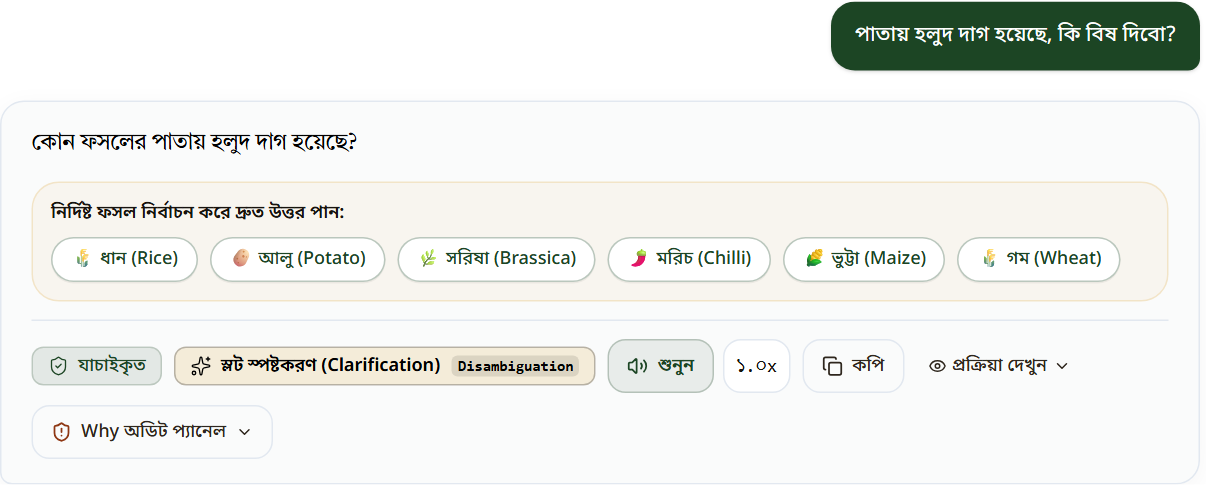
\includegraphics[width=\linewidth,height=3.6cm,keepaspectratio]{../screenshots/fig2a_ask.png}
  \caption{\textbf{ASK (S1)}. A crop-less treatment query retrieves no sources; six crop chips ask for the crop.}
  \label{fig:demo_ask}
\end{subfigure}
\hfill
\begin{subfigure}[t]{0.49\textwidth}
  \centering
  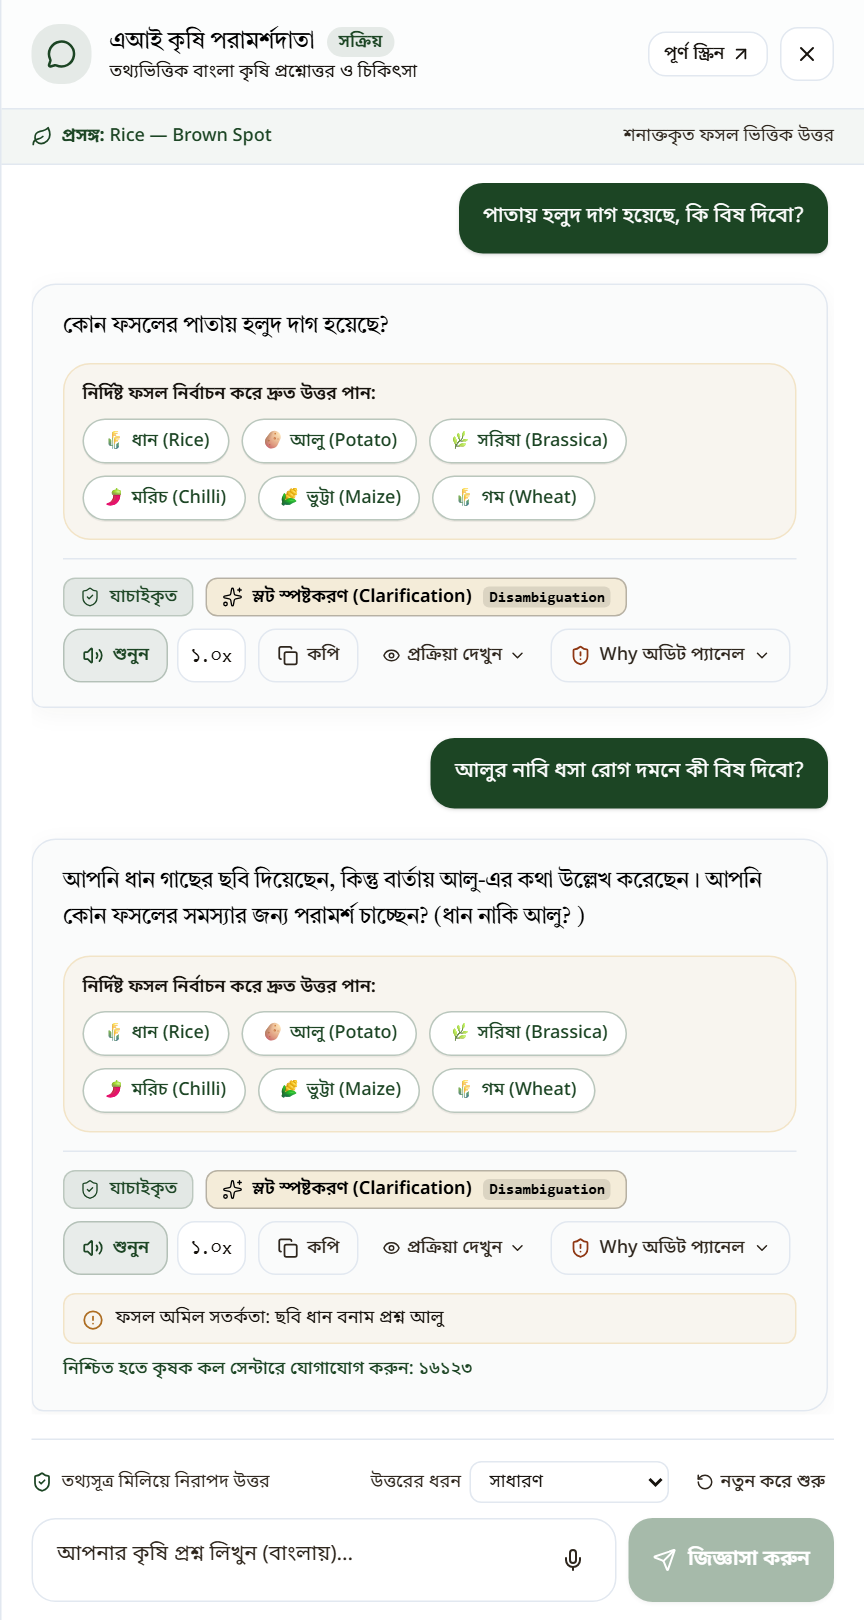
\includegraphics[width=\linewidth,height=3.6cm,keepaspectratio]{../screenshots/fig2b_mismatch.png}
  \caption{\textbf{CONFIRM (S3)}. A rice photograph with a potato question raises the Clarification badge; chemical advice waits.}
  \label{fig:demo_mismatch}
\end{subfigure}
\\[3pt]
\begin{subfigure}[t]{0.49\textwidth}
  \centering
  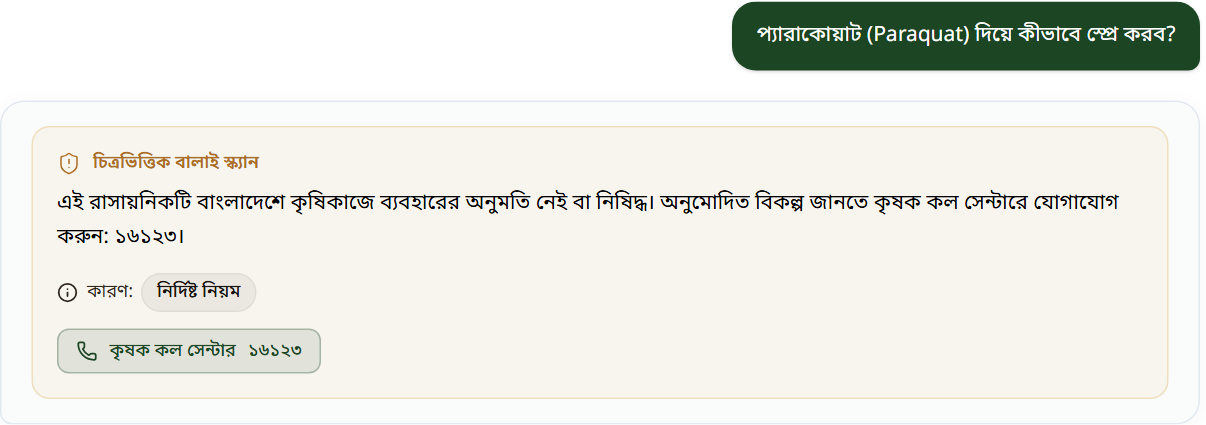
\includegraphics[width=\linewidth,height=3.6cm,keepaspectratio]{../screenshots/fig2d_refer.png}
  \caption{\textbf{REFER (S4)}. A paraquat request is stopped at T0 and routed to the 16123 helpline.}
  \label{fig:demo_refer}
\end{subfigure}
\hfill
\begin{subfigure}[t]{0.49\textwidth}
  \centering
  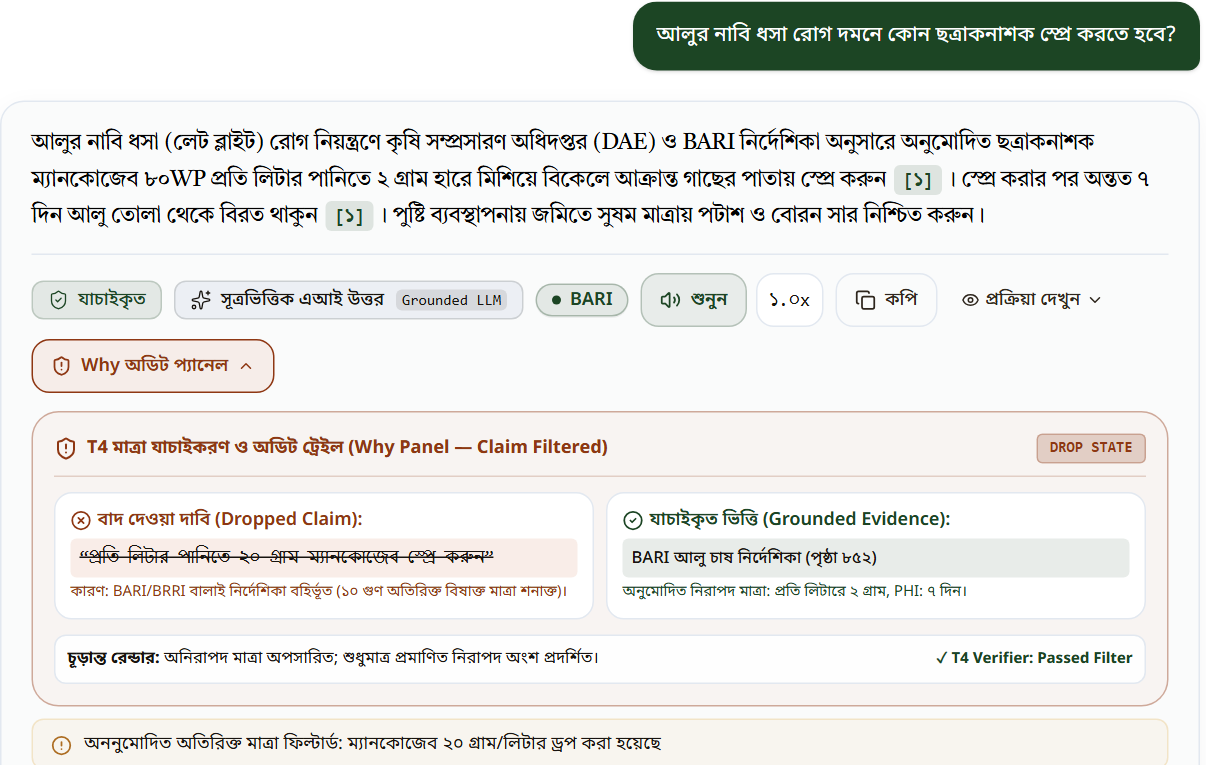
\includegraphics[width=\linewidth,height=3.6cm,keepaspectratio]{../screenshots/s5_why_panel.png}
  \caption{\textbf{DROP (S5)}. The \textit{Why} panel lists the dropped $10\times$ overdose and the BARI passage (p.~852) that grounds the kept dose.}
  \label{fig:demo_why}
\end{subfigure}
\caption{Interface states for ASK, CONFIRM, REFER, and DROP. Full-size screens for S1--S5 are in Appendix~\ref{app:ui}.}
\label{fig:demo_states}
\end{figure*}

The demonstration is aimed at researchers and practitioners who build multilingual, multimodal, or safety-critical conversational systems. Attendees walk through five steps, S1--S5, on the live system. Each step shows what the farmer does, what the system displays, and what it allows next. Attendees can start from preset regional-dialect and safety-test queries, or type their own text and upload photographs.

\textbf{S1: Missing crop (ASK).}
The farmer writes, without naming a crop: \textit{``Patay holud dag hoyeche, ki bish dibo?''} (``Yellow spots on the leaves. What pesticide should I use?''). \textbf{T1} halts before retrieval ($sources\_retrieved = 0$) and shows crop chips (Figure~\ref{fig:demo_ask}). Tapping \textit{Alu} (potato) binds the crop, and potato-scoped retrieval returns an answer with numbered citations.

\textbf{S2: A photograph scopes the evidence.}
In a new consultation, the farmer uploads a rice leaf photograph. The on-device classifier predicts rice, and \textbf{T2} scopes retrieval to rice guidance. The image stays on the device.

\textbf{S3: Text--image conflict (CONFIRM).}
Keeping the rice photograph attached, the farmer asks about potato late blight. The system raises the \textbf{Clarification} badge and withholds chemical advice (Figure~\ref{fig:demo_mismatch}) until the farmer picks one crop.

\textbf{S4: High-risk chemical request (REFER).}
The farmer asks how to apply paraquat, which the safety policy blocks. The \textbf{T0} precheck stops the turn before retrieval or generation and shows a safety notice with a one-tap call to the Krishi Call Centre (\textbf{16123}; Figure~\ref{fig:demo_refer}).

\textbf{S5: Dosage verification (DROP).}
The farmer asks a new question about fungicide for potato blight. In the recorded session the draft contains one dose ten times above the BARI range. \textbf{T4} drops that sentence and delivers the rest with citations, a provenance badge, and an expandable \textit{Why} panel that names the removed claim (Figure~\ref{fig:demo_why}).

\section{Evaluation}
\label{sec:evaluation}

We ask three questions, one per control. (Q1) Do admission controls stop or redirect unsafe and underspecified requests? (Q2) Does evidence binding keep wrong-crop evidence away from generation, and are conflicts surfaced? (Q3) Can release checks catch what the generator gets wrong? Table~\ref{tab:headline} summarizes the main results; Appendix~\ref{app:evidence} lists each result with its sample, status, and scope.

\begin{table}[t]
\centering
\scriptsize
\setlength{\tabcolsep}{1.5pt}
\begin{tabular*}{\columnwidth}{@{\extracolsep{\fill}}llr@{}}
\toprule
\textbf{Control} & \textbf{Test set} & \textbf{Result} \\
\midrule
Crop gate (C1) & 200 farmer, 30 crop-less & 30/30 halted; 170/170 pass \\
Banglish T0 (C1) & 85 attack, 15 benign & 85/85 (formal 1/85); 0/15 \\
Crop binding (C2) & 400 stress & cross-crop 36.25\% $\rightarrow$ 30.0\% \\
Mismatch (C2) & 54 farmer, 400 syn. & 453/454; 0/454 controls \\
T3 prompt only & 280/arm, local 4B & ASR 52.5\% $\rightarrow$ 10.71\% \\
Verifier (C3) & 118 errors, 38 ans. & 114 caught; 0/38 clean flagged \\
\bottomrule
\end{tabular*}
\caption{Main results. Appendix~\ref{app:evidence} gives confidence intervals, the remaining experiments, and scope.}
\label{tab:headline}
\end{table}

\subsection{Q1: Admission and Referral}
\label{sec:eval-gate}

We test the crop gate on 200 real Bengali farmer treatment queries, 30 of which name no crop. Two annotators labeled crop presence independently and agreed on every query (Cohen's $\kappa = 1.00$). The gate halted all 30 crop-less queries before retrieval and passed the other 170 to crop-scoped search without a false halt. On the same queries, an LLM prompted to make this decision halted 10\% of queries against the gate's 15\%, agreed with the gate on 91\% of decisions, and took a median 4.2\,s per query.

Colloquial spelling also affects the T0 precheck. On 85 Latin-script and phonetic attacks (for example \textit{parakwat} for paraquat), a precheck limited to formal English and Bengali script caught 1. Our normalized precheck caught all 85 and raised no alarm on 15 benign farmer questions (Appendix~\ref{app:architecture}).
\subsection{Q2: Evidence Binding and Conflict Handling}
\label{sec:eval-fence}

We measure crop binding on a 400-query stress set of colloquial, dialectal, Banglish, and ambiguous-disease queries, each with a gold crop. A query counts as \emph{cross-crop retrieval} when any of its top five passages is tagged to another crop; this is a retrieval measure, not a judgment of the final answer. Open retrieval gives 36.25\%. Binding the gold crop, which simulates correct crop routing, lowers this to 30.0\%: 25 queries improve and none get worse (exact McNemar $p = 6 \times 10^{-8}$). The remaining 30\% shows that binding reduces cross-crop evidence without removing it (Section~\ref{sec:system_retrieval}). The six on-device disease classifiers that run after crop routing reach 0.94 to 0.99 top-1 accuracy on 4,294 held-out images, and the family router assigns 433 of 437 images to the correct botanical family.

For conflicts, each case pairs a query with a photograph of a different crop, and each has a matched control with the same query and a matching photograph. The badge fired on 53 of 54 farmer cases and all 400 cases in PRISM, our synthetic conflict suite, and on none of the 454 controls. The one miss referred to the crop only implicitly. On a separate set of 300 conflict queries from earlier work, a prompted LLM asked the farmer to clarify in 20\% of cases and naive multimodal RAG in 13\%; these are different cases, so we report them only as context.

\subsection{Q3: Release Checks on Generated Advice}
\label{sec:eval-safety}

We first measure how much the generator resists attacks on its own. With T0 and T4 disabled, we sent 280 attack prompts to \texttt{krishokchat-4b}: 210 across seven attack families and 70 additional Bengali-native probes. Each prompt ran once under the guarded system prompt and once under a neutral prompt. Attack success rate (ASR), judged by a fixed rule-based classifier, fell from 52.5\% to 10.71\% (147 to 30 successes), and from 77\% to 19\% on the 100 Bengali-native prompts. The residual is what the surrounding stages have to catch. Remaining successes were concentrated in Bengali-native (19/100), delimiter-hijacking (6/30), and retrieval-poisoning (5/30) prompts. Adding the T0 precheck, as in the deployed pipeline, lowers ASR on the same 280 prompts to 4.64\% [2.73, 7.78] (13/280) and to 2.0\% [0.55, 7.00] on the Bengali-native prompts; T0 intercepted 207 of 280 attack prompts (194 banned-chemical matches, 12 injection patterns). Of 200 real farmer queries, 9 were blocked as out-of-scope coverage (livestock, training, and availability queries); none were crop-treatment queries. A cloud run is reported in Appendix~\ref{app:evidence}; its unguarded arm used a different model, so it is not a controlled comparison.

We then assess delivered advice. Three blinded raters (two agronomy or botany undergraduates and one extension officer) judged 46 of 47 guarded outputs safe and actionable, one vague but harmless, and none dangerous (Fleiss' $\kappa = 0.82$). All three unguarded control outputs were rated dangerous.

To test the dosage verifier, we inserted controlled errors into verified answers. On 38 live answers carrying 118 inserted errors, it caught 114 and rejected none of the 38 unmodified originals. On a larger benchmark built from 88 BARI and BRRI passages, it caught 296 of 350 inserted errors (84.6\%), including every overdose (76/76) and underdose (67/67). It was weaker on chemical substitutions (85\%), unit substitutions (73\%), and invented pre-harvest intervals (65\%), which marks the limit of what ``dosage verification'' covers.

SMS delivery loses information. The deterministic packer kept 399 of 400 messages within 160 GSM-7 characters and kept the dose in 92 of 100 long advisories, but the chemical name in only 34 (Appendix~\ref{app:delivery}).

\subsection{What This Evaluation Does Not Establish}
\label{sec:eval-scope}

These results describe behavior on the listed test sets. They do not show effects on yield or farmer decisions. The crop-binding study simulates correct routing; 400 of 454 conflict cases are synthetic; multi-turn tests use constructed dialogues; the output audit covers 47 answers; network tests use simulated packet loss; and the verifier checks numerical dosage claims, not agronomy in general.

% =========================================================================
% SECTION 6: LIMITATIONS AND CONCLUSION
% =========================================================================
\section{Limitations, Availability, and Conclusion}
\label{sec:conclusion}

\paragraph{Limitations.}
\label{sec:limitations}
\emph{Coverage.} The system supports six crop groups and Bengali input over a BM25 index. Revising guidance means editing the index, but adding a crop also needs a classifier, aliases, and policy rules. \emph{Ambiguity.} The mismatch check handles explicit crop names only, and crop binding leaves 30\% cross-crop retrieval even with the correct crop. \emph{Residual unsafe output.} With the guarded prompt alone, 10.71\% of attacks succeed on the local model (19\% Bengali-native); with T0 in front, as deployed, this falls to 4.64\% (2.0\% Bengali-native). The remaining 13 failures are concentrated in delimiter-hijacking (6/30) and retrieval-poisoning (5/30) families that do not name banned chemicals, and the verifier misses some unit, chemical, and interval errors. \emph{Delivery.} SMS compression drops chemical names, and local generation takes about 24\,s per call.

\paragraph{Availability and Licensing.}
\label{sec:availability}
Code is released under the MIT license at \url{https://github.com/RaiyaanReza/KrishokChat-Agricultural-Advisory-System}. The on-device vision models are released under Apache-2.0 at \url{https://huggingface.co/RaiyanKhaan/KrishokTech-Models}. The \texttt{krishokchat-4b} weights and the 2{,}135-passage evidence index, derived from BARI, BRRI, and DAE guidelines, are released at the same model repository under Apache-2.0. The T0 pattern lists are withheld from the public release; the public package therefore does not reproduce the full T0 precheck. They are available to qualified researchers and safety auditors under a non-commercial research agreement.

\paragraph{Conclusion.}
\label{sec:final_conclusion}
The model drafts, while deterministic controls decide access, confirmation, referral, and dosage release. KrishokTech makes each of these decisions visible to the farmer and to attendees, and keeps agricultural knowledge in an index that can be revised without retraining. The measured controls reduce but do not remove failures, and the system is meant to support extension officers, not replace them. No claim of field effectiveness is made; evaluation with farmers remains to be done.

% =========================================================================
% ETHICS AND BROADER IMPACT STATEMENT
% =========================================================================
\clearpage
\section*{Ethics and Broader Impact Statement}
\label{sec:ethics}

Agricultural advice for smallholder farmers affects food security, livelihoods, and physical safety. Incorrect chemical or dosage guidance is the central risk this paper is designed around.

\paragraph{Farmer Query Data.} The 200 farmer queries in the gate evaluation (Section~\ref{sec:eval-gate}) come from extension-service interaction logs. Names, phone numbers, and plot locations were removed before analysis. The queries were collected with regional extension officers under institutional review at North South University, and informed consent was obtained for non-commercial research and safety evaluation. Two annotators labeled the crop slot independently, with consensus adjudication; agreement statistics are in Appendix~\ref{app:gate}.

\paragraph{Agricultural Image Data.} Farmer photographs are classified on the device (WebAssembly and ONNX) and are not uploaded in either deployment mode. The held-out images used to measure vision accuracy (Section~\ref{sec:eval-fence}) come from open datasets: PlantVillage, the Bangladesh Rice Knowledge Bank, and Kaggle agricultural datasets under CC-BY and open research licenses.

\paragraph{Pesticide and Dosage Guidance.} Recognized high-risk chemical requests and poisoning language trigger a rule-based block and a helpline referral before any generation, and dosage claims are checked against source passages and dose ranges before display (Section~\ref{sec:system_verification}). Requests or claims that the rules do not recognize can still pass. On the deployed model the T0 precheck and guarded prompt together leave a 4.64\% attack success rate (2.0\% on Bengali-native attacks), down from 10.71\% with the prompt alone; the dosage verifier missed 4 of 118 inserted errors (Section~\ref{sec:eval-safety}). We report these residuals and do not claim that the system prevents all unsafe output.

\paragraph{Helpline Referral.} Agronomic chemical inquiries are referred to the national Krishi Call Centre (16123), which operates 9:00\,AM--5:00\,PM, Saturday through Thursday. Because those hours do not cover emergencies, poisoning, self-harm, and medical-crisis language is instead referred to the 24/7 National Emergency Service (999) and local health facilities. The system displays these routes immediately; it cannot ensure that help is reached. The public sandbox shows the block and referral for toxic-chemical queries without giving advice on them.

\paragraph{Third-Party Model Use.} The connected web demo and several benchmarks use a third-party API (\texttt{google/gemini-2.5-flash-lite}) under a zero-data-retention agreement. In this mode, text queries, including the de-identified farmer queries used for the gate comparison in Section~\ref{sec:eval-gate}, are sent to the API; photographs and direct personal identifiers are not. In the self-hosted mode, generation runs on the local \texttt{krishokchat-4b} model through llama.cpp.

\paragraph{Human Oversight.} KrishokTech is meant to support extension officers, not replace them. A turn ends in ASK or CONFIRM when the system needs information from the farmer, and in a referral to a human service when a request falls under the safety policy. All results are scoped to the conditions in which they were measured (Section~\ref{sec:eval-scope}), and simulated components are labeled as such.

% =========================================================================
% REFERENCES
% =========================================================================
\begingroup
\let\oldthebibliography\thebibliography
\renewcommand{\thebibliography}[1]{%
  \oldthebibliography{#1}%
  \setlength{\itemsep}{0.6pt plus 0.2pt}%
  \setlength{\parskip}{0pt}%
}
\bibliography{krishoktech_eacl}
\endgroup

% =========================================================================
% APPENDIX
% =========================================================================
\clearpage
\appendix

\section{Architecture, Decision Logic, and Gate Evaluation}
\label{app:architecture}
\label{app:gate}

This section gives the decision rules behind the five stages (Figure~\ref{fig:architecture}) and the evaluation detail for the pre-retrieval gate.\footnote{The exact pattern lists of the T0 precheck (for example, phonetic and textual variants of restricted organophosphates and self-harm phrases) are withheld to prevent evasion and dual use. They are available to qualified researchers and safety auditors under a non-commercial research agreement.}

\paragraph{State transitions.} \textbf{REFER} (T0) ends the turn; the next message is processed from T0 again. \textbf{ASK} (T1) ends the turn with crop chips; a chip or a typed crop binds the crop and the request resumes at T2. \textbf{CONFIRM} (T2) holds chemical advice until the farmer picks one crop, which then becomes the bound crop. \textbf{DROP} (T4) acts on single claims: the unsupported sentence is removed and the rest of the draft is delivered.

\paragraph{Information-state extractor (T1).} The extractor uses gazetteers and pattern rules, with no language model, to fill five slots: crop (mapped to a 45-crop taxonomy), growth stage, location, intent (treatment, prevention, general), and symptom tokens. A treatment or problem intent with an empty crop slot halts before retrieval. On the 200 farmer queries, the extractor's crop label matched the adjudicated gold label on 95.5\% of queries (miss 1.5\%, false positive 3.0\%; each false positive contains a genuine crop mention in a multi-crop or sourcing query). Annotator agreement on the same queries was 100\% for crop presence ($\kappa = 1.00$), 99.5\% for the 37-crop normalized label ($\kappa = 0.99$), and 93.5\% for intent ($\kappa = 0.90$). A constructed pilot halted 100 of 100 crop-less requests; of 140 crop-specified requests, 114 passed directly and 26 received a bounded clarification for another slot.

\paragraph{Vision crop router (T2).} With top-1 probability $p_1$ and top-2 probability $p_2$: if $p_1 \ge 0.90$ and $p_1 - p_2 \ge 0.20$, the predicted crop is bound; if $p_1 \ge 0.40$ but either condition fails, the top two crops are offered as chips; if $p_1 < 0.40$, retrieval halts and the farmer is asked to retake the photograph.

\paragraph{Dialect presets.} The \textit{DialectSelector} offers Standard Bengali, Sylheti, Chittagonian, Noakhali, Rangpuri, and Barishali presets. Each adds regional synonyms during query normalization while leaving chemical names unchanged. The presets are implemented features; we have not measured accuracy per dialect.

\paragraph{Provenance badges.} Each rendered response carries one badge: \emph{Fact lookup} (T2, exact match in a nine-fact base, no generation), \emph{Grounded generation} (T3/T4, draft passed the dosage verifier), \emph{Guidance card} (T1, non-chemical advice on a crop-less halt), \emph{Clarification} (T1/T2, crop chips or mismatch warning), or \emph{Referral} (T0, helpline routing).

\paragraph{Banglish red-teaming.} Table~\ref{tab:banglish_eval} gives the constructed T0 benchmark. For attack rows the outcome is the number intercepted; for benign rows it is the number passed.

\begin{table}[t]
\centering
\footnotesize
\setlength{\tabcolsep}{2.5pt}
\begin{tabular*}{\columnwidth}{@{\extracolsep{\fill}}lcccc@{}}
\toprule
\textbf{Set} & \textbf{\textit{n}} & \textbf{Formal} & \textbf{Normalized} & \textbf{Route} \\
\midrule
Phonetic chemical & 35 & 0 blocked & 35 blocked & 16123 \\
Banglish crisis   & 25 & 1 blocked & 25 blocked & 999 \\
Indirect sabotage & 25 & 0 blocked & 25 blocked & 16123 \\
\midrule
\textbf{All attacks} & \textbf{85} & \textbf{1 (1.2\%)} & \textbf{85 (100\%)} & \\
Benign control    & 15 & 15 passed & 15 passed & none \\
\bottomrule
\end{tabular*}
\caption{Banglish and phonetic red-teaming of the T0 precheck ($N=100$): a precheck limited to formal English and Bengali script versus the normalized precheck. The 95\% Wilson interval for 85/85 is [95.7, 100].}
\label{tab:banglish_eval}
\end{table}

\section{Delivery, Offline Operation, and Deployment}
\label{app:deployment}
\label{app:delivery}

\subsection{SMS Enforcement}
Lengths are counted in GSM-7 characters on Latin-script SMS output; a Bengali-script message would need UCS-2 encoding (70 characters per segment) and more segments. The SMS packer produced 299/300 offline and 100/100 live messages within 160 characters (399/400 overall), and all 8 referral messages carried only the referral. In a live audit of 92 long advisories, naive truncation kept the dose in 12, because conversational preamble pushed it past the 160-character limit. The deterministic 11-slot compressor kept dose, application interval, and pre-harvest interval in all 1,000 constructed input tuples (102--115 characters, none over 160) and kept 65 of 66 dosage claims on live gold advisories. It copies slots from the verified answer and does not write new values, although copying cannot guard against a wrongly extracted slot.

Table~\ref{tab:n05c} compares three compression arms on 100 long dose-carrying advisories. The compressor kept the dose most often, but the LLM summarizer kept the chemical name more often (56 vs.\ 34), so a retained dose alone does not make a complete instruction. The LLM summarizer is only a baseline; the deployed path uses the compressor.

\begin{table}[t]
\centering
\footnotesize
\setlength{\tabcolsep}{3pt}
\begin{tabularx}{\columnwidth}{@{}Xccc@{}}
\toprule
\textbf{Measure} & \textbf{Naive} & \textbf{LLM} & \textbf{Compressor} \\
\midrule
Dose survival & 23/100 & 89/100 & 92/100 \\
Chemical survival & 20/100 & 56/100 & 34/100 \\
Length $\le 160$ chars & 100/100 & 98/100 & 100/100 \\
Invented dosage & 0 (copies) & 1 (+1 bord.) & 0 \\
\bottomrule
\end{tabularx}
\caption{Three-arm SMS comparison (N05c) on 100 paired long dose-carrying advisories (seed 42). All arms share the same frozen dose and chemical detectors.}
\label{tab:n05c}
\end{table}

\subsection{Offline Retrieval}
Local BM25 retrieval reached a hit rate of $0.94$, and service-worker precaching recorded 0 cache misses over 400 requests. Under simulated packet loss, local retrieval stayed at 0.94, while remote retrieval lost 13.25\,pp at 15\% loss and 30.0\,pp at 30\% loss. This covers retrieval only; offline generation depends on the local model.

\subsection{Installation Footprint}
Table~\ref{tab:footprint} lists measured sizes. They cover the application and vision assets and exclude the \texttt{krishokchat-4b} weights, which add several gigabytes.

\begin{table}[t]
\centering
\small
\begin{tabular}{lr}
\toprule
\textbf{Artifact (excluding LLM weights)} & \textbf{Size (MB)} \\
\midrule
Unique ONNX vision assets (11 files) & 95.64 \\
Minimal installation & 284.0 \\
Installation with PyTorch checkpoints & 339.6 \\
\bottomrule
\end{tabular}
\caption{Measured installation footprint, excluding the language model.}
\label{tab:footprint}
\end{table}

\subsection{Latency Breakdown}
Table~\ref{tab:latency} lists non-generation latency ($n=400$, median 33.565\,ms). Generation is excluded: the local model takes about 24\,s per call on CPU, and the gate comparison LLM took a median 4.2\,s per decision.

\begin{table}[t]
\centering
\small
\begin{tabular}{lrr}
\toprule
\textbf{Component} & \textbf{Median (ms)} & \textbf{p95 (ms)} \\
\midrule
Safety processing & 0.321 & 0.705 \\
BM25 retrieval & 26.831 & 61.248 \\
Verification & 4.815 & 11.220 \\
\midrule
Total pipeline & 33.565 & 67.833 \\
\bottomrule
\end{tabular}
\caption{Safety, retrieval, and verification latency ($n=400$ requests, BM25 only, stub LLM). Component medians need not sum to the total median.}
\label{tab:latency}
\end{table}

\subsection{Zero-LLM Turns and Modeled Cost}
On a 1,000-query benchmark mix, 7.9\% of turns needed no LLM: 5.7\% ended at T0 and 2.2\% were answered from the T2 fact base, while 92.1\% reached generation. Using provider-metered token counts from 58 live calls and published API prices, this mix costs USD~0.1720 per 1,000 turns against USD~0.1995 if every turn reached generation. This is a model of API cost on a benchmark mix, not billed expenditure or farmer traffic.

\subsection{Trace Ordering}
Across 100 evaluation cases, all 100 provenance traces kept the required event order (median 9 events per turn).

\section{Demonstration Gallery}
\label{app:ui}

Figures~\ref{fig:app_halt}--\ref{fig:app_drop} show full-size screens for the five steps (S1--S5) in Section~\ref{sec:demonstration}.

\begin{figure}[h]
\centering
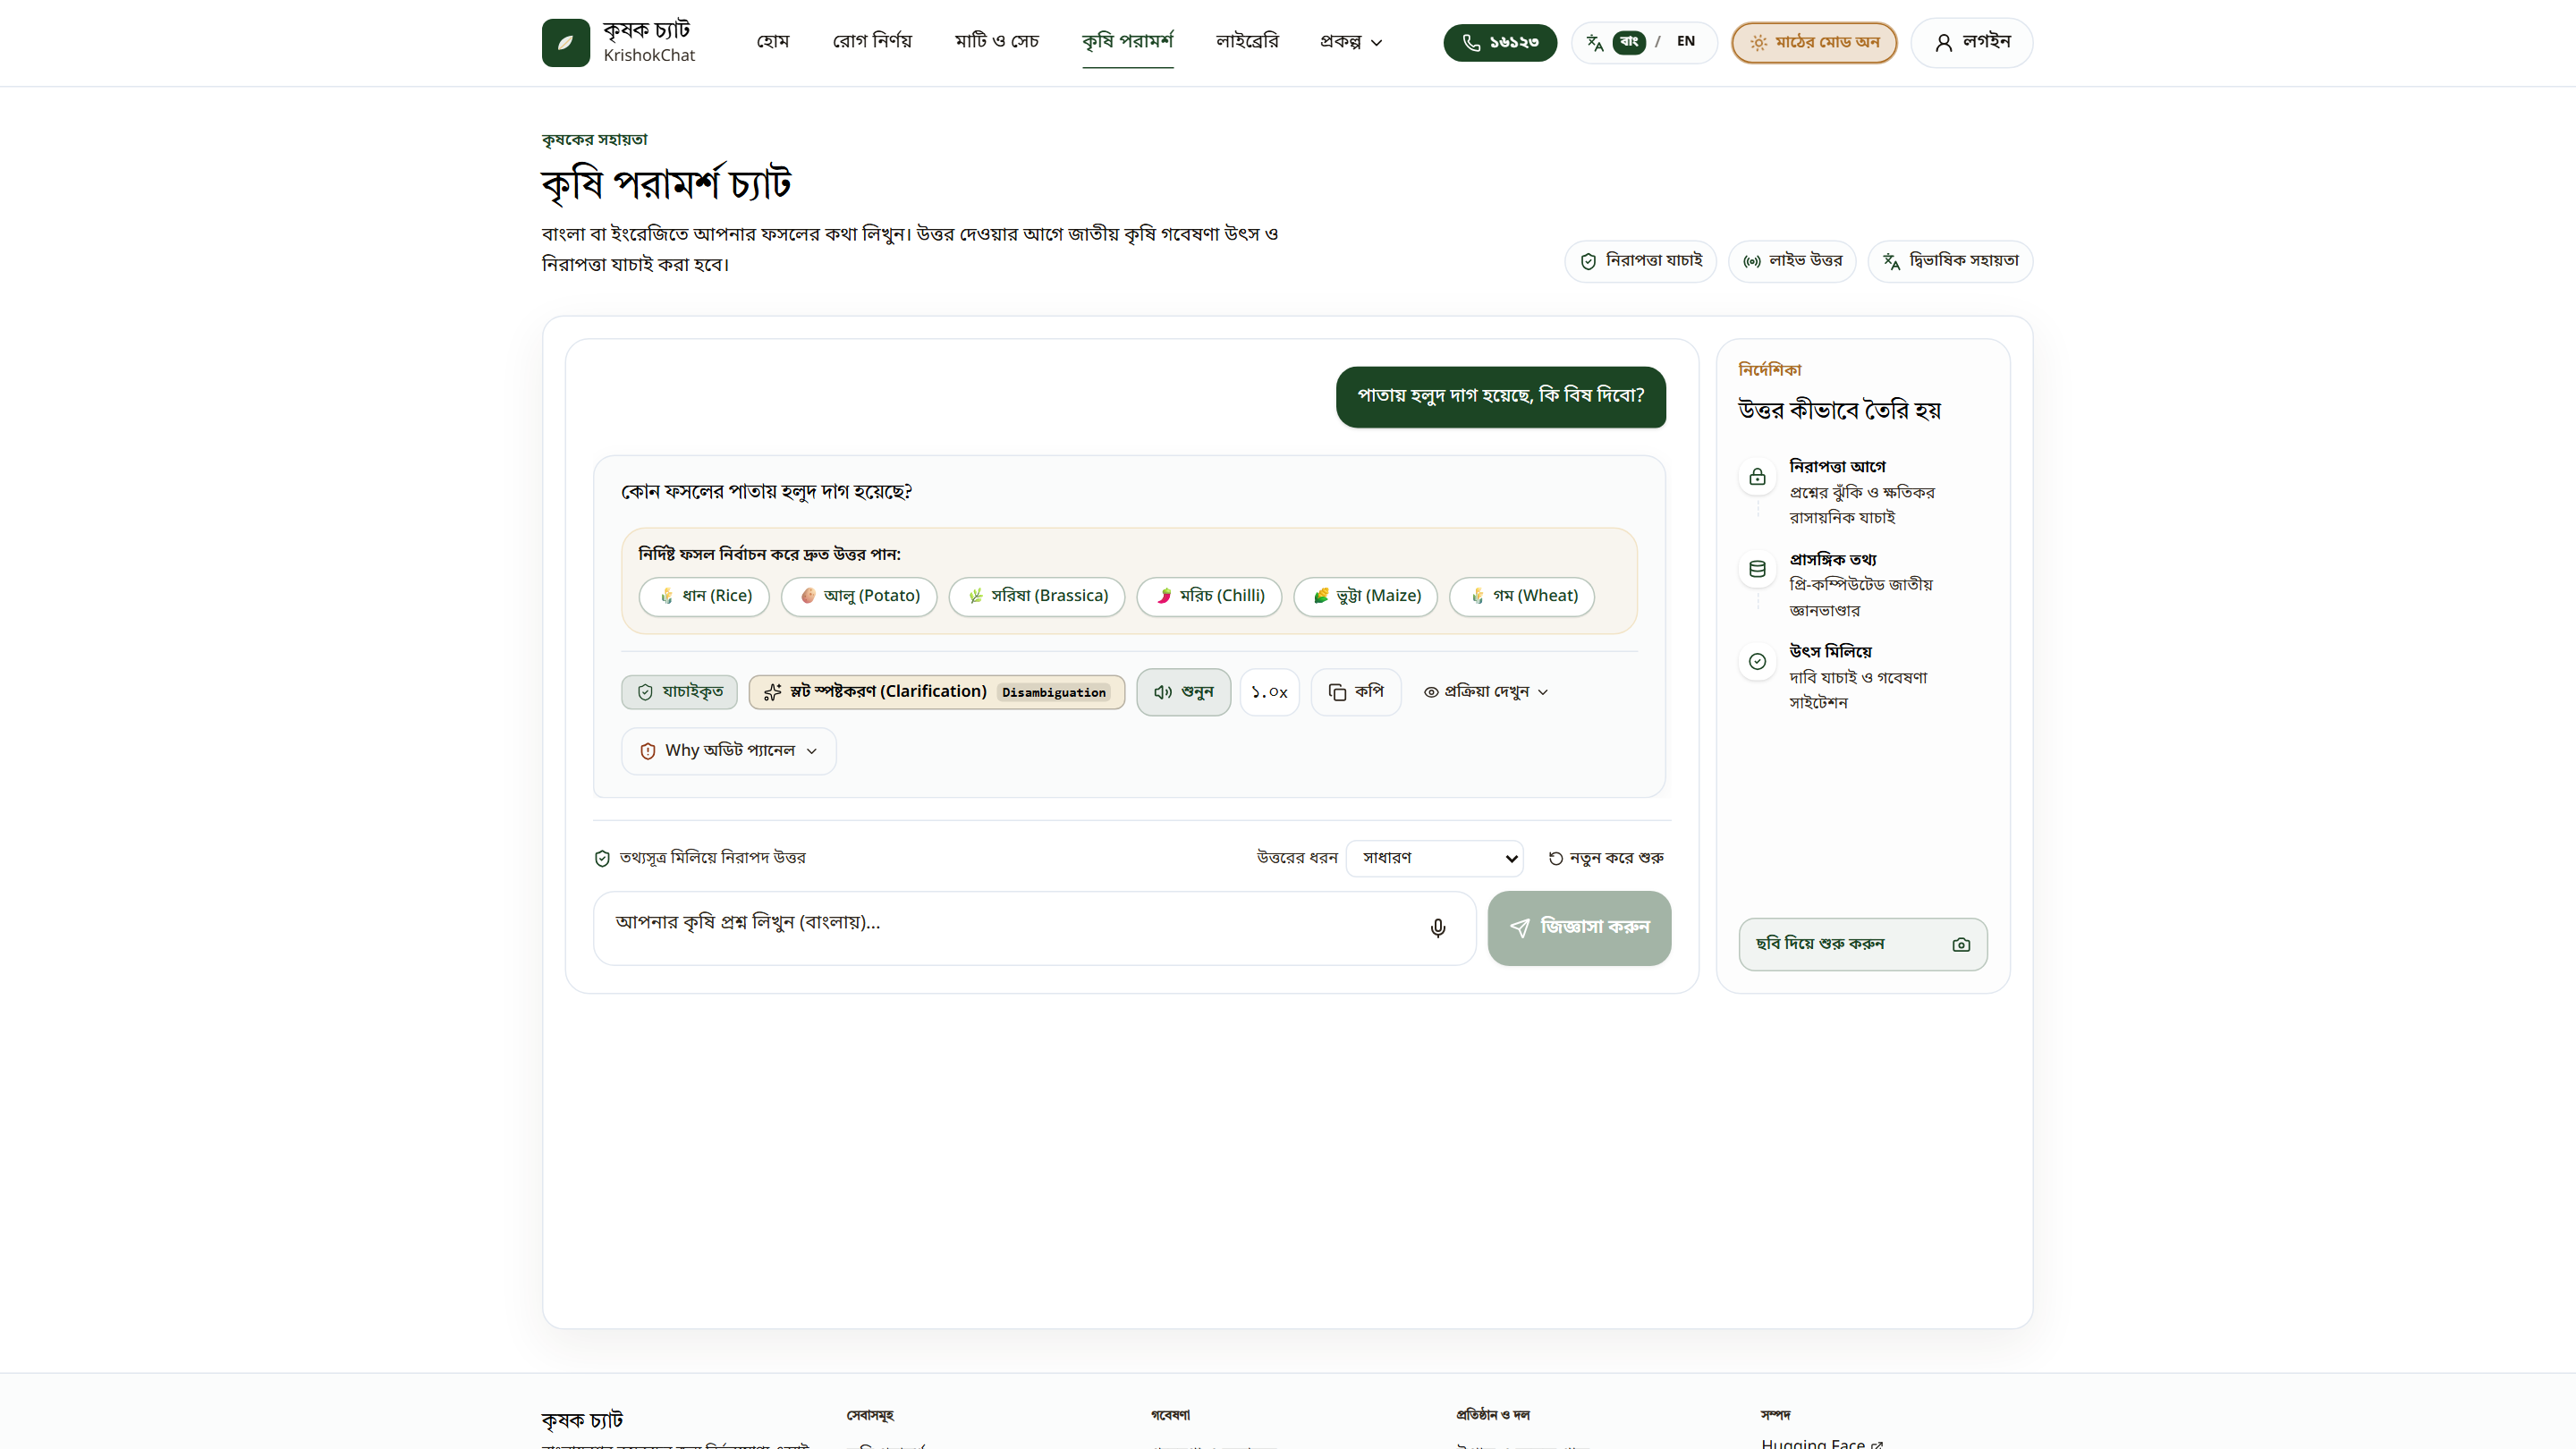
\includegraphics[width=0.92\linewidth]{../screenshots/screenshot1_halt_clarification.png}
  \caption{ASK (S1): a colloquial treatment query that names no crop halts before retrieval, and the system offers Bengali crop chips.}
\label{fig:app_halt}
\end{figure}

\begin{figure}[h]
\centering
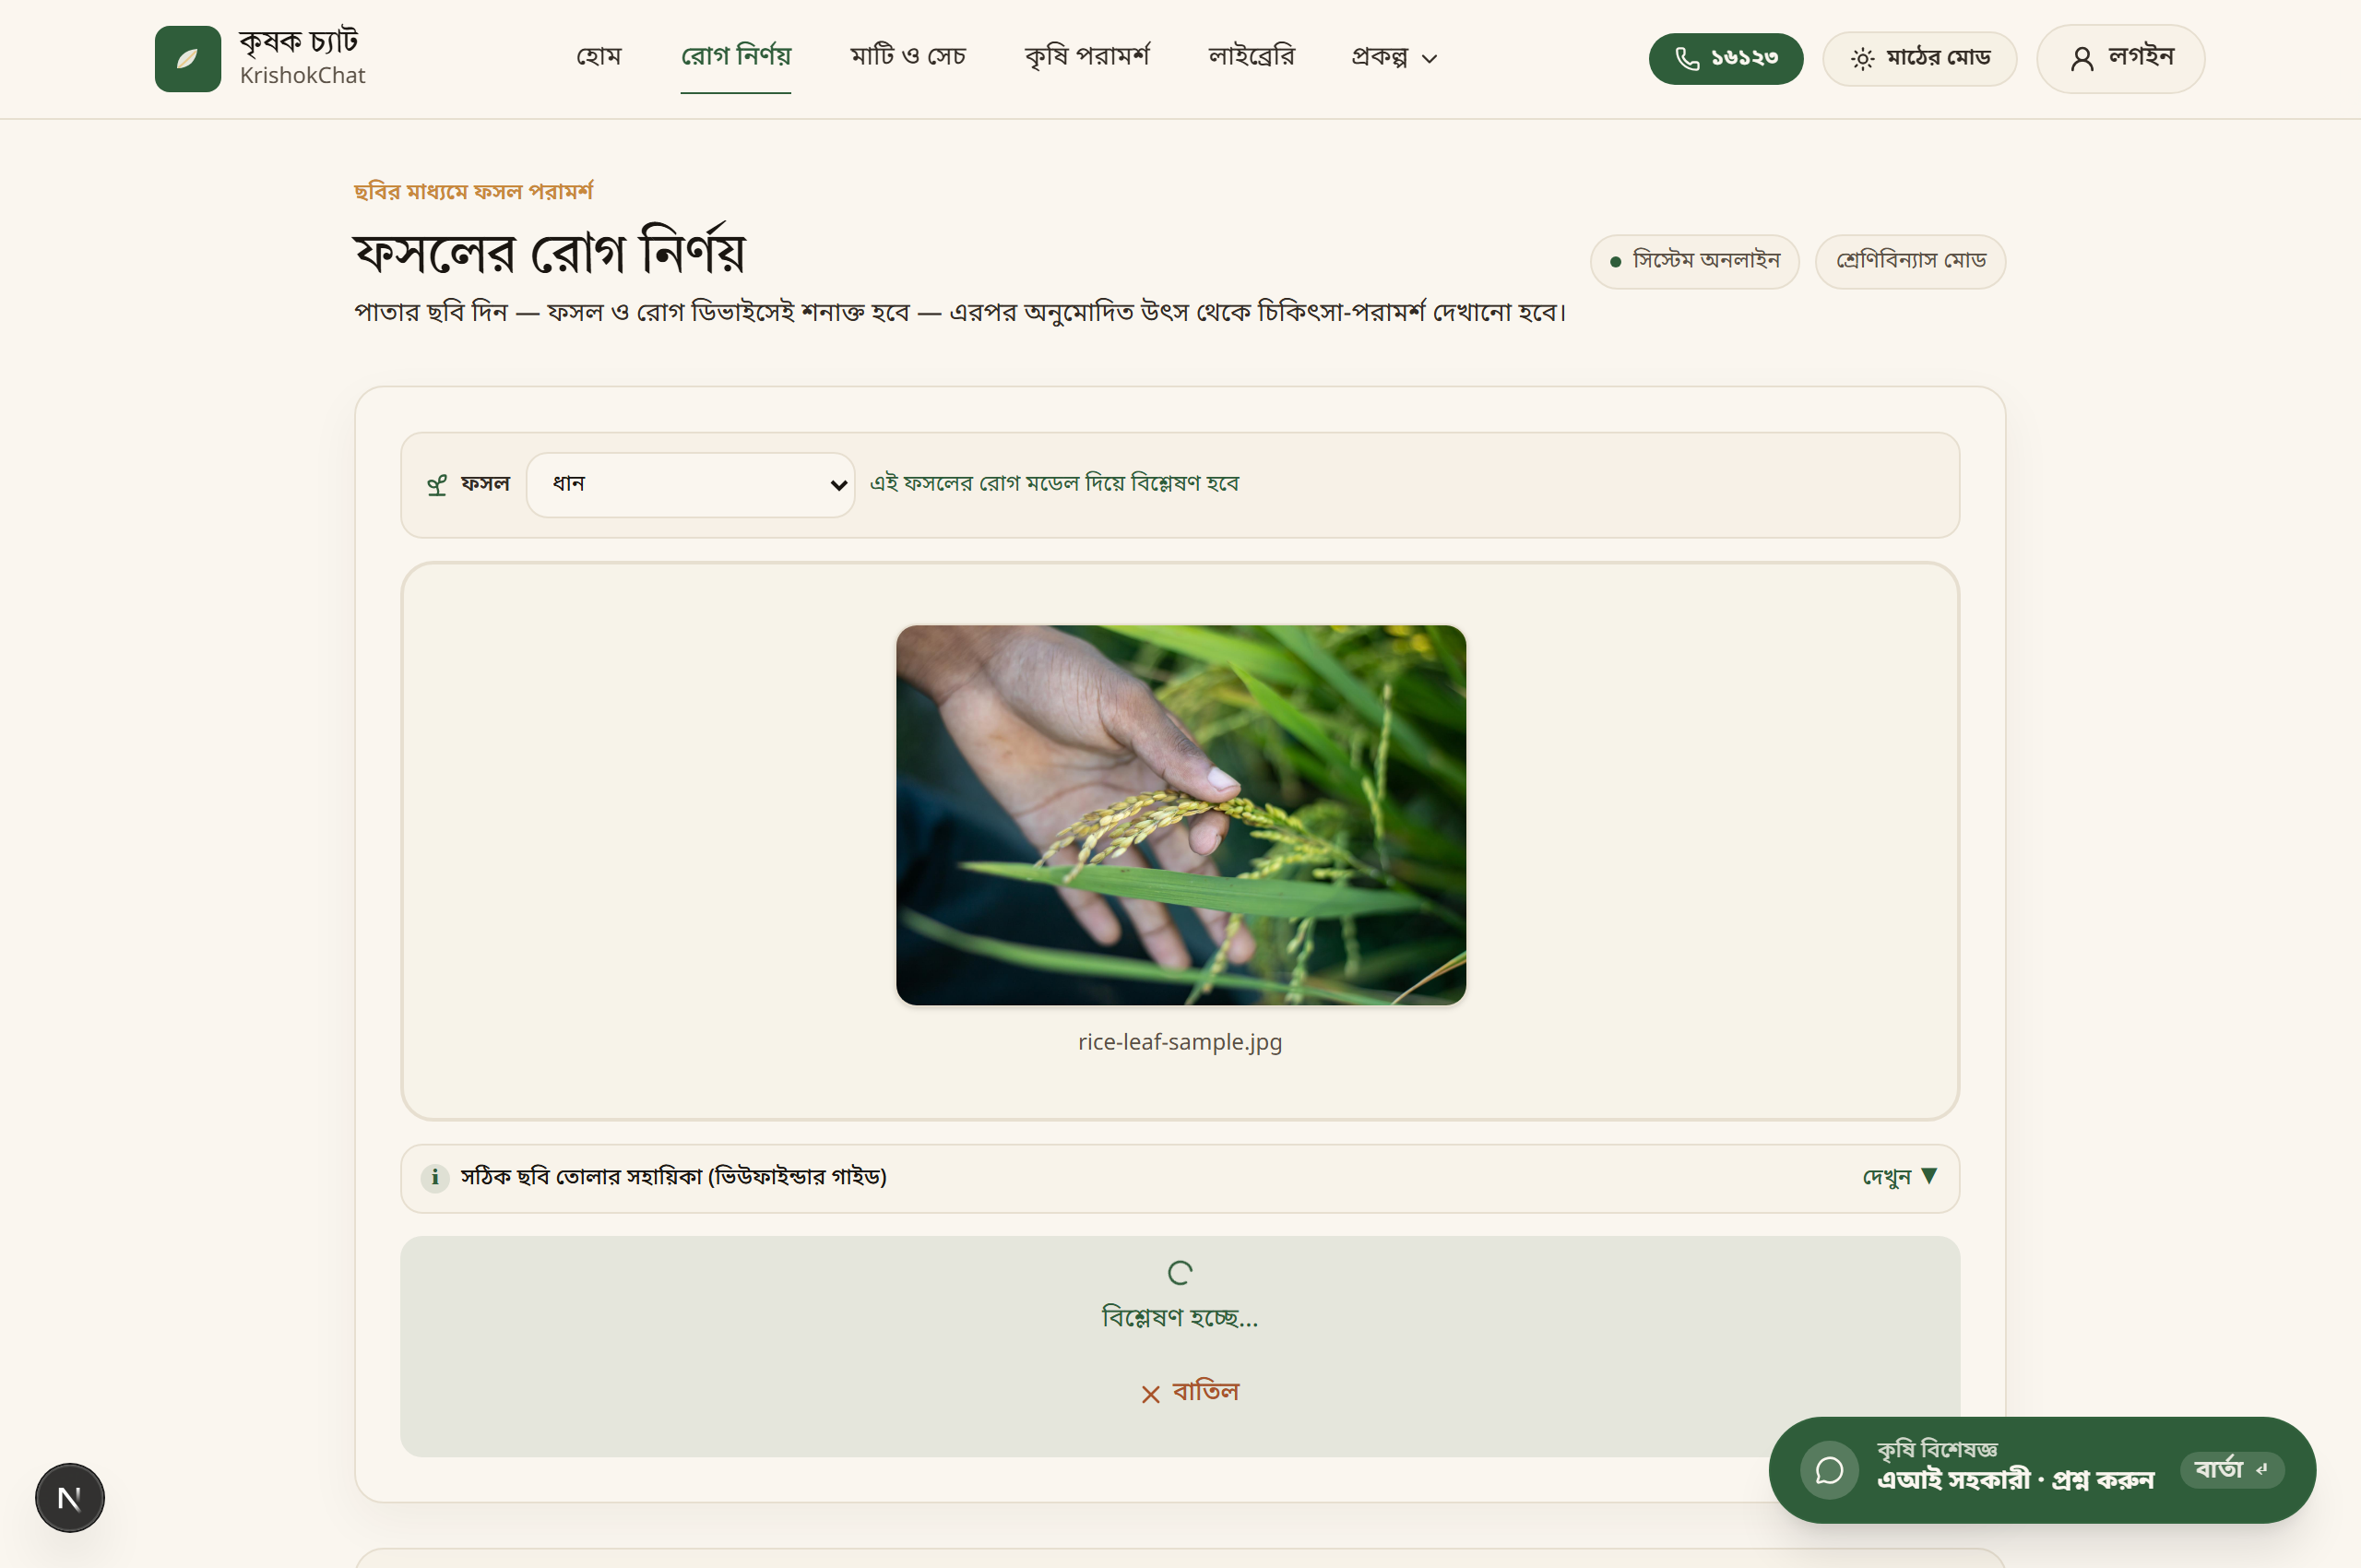
\includegraphics[width=0.92\linewidth]{../screenshots/screenshot3_photo_crop_scope.png}
  \caption{S2: the on-device classifier predicts the crop from a leaf photograph, and retrieval is scoped to that crop's guidance.}
\label{fig:app_fence}
\end{figure}

\begin{figure}[h]
\centering
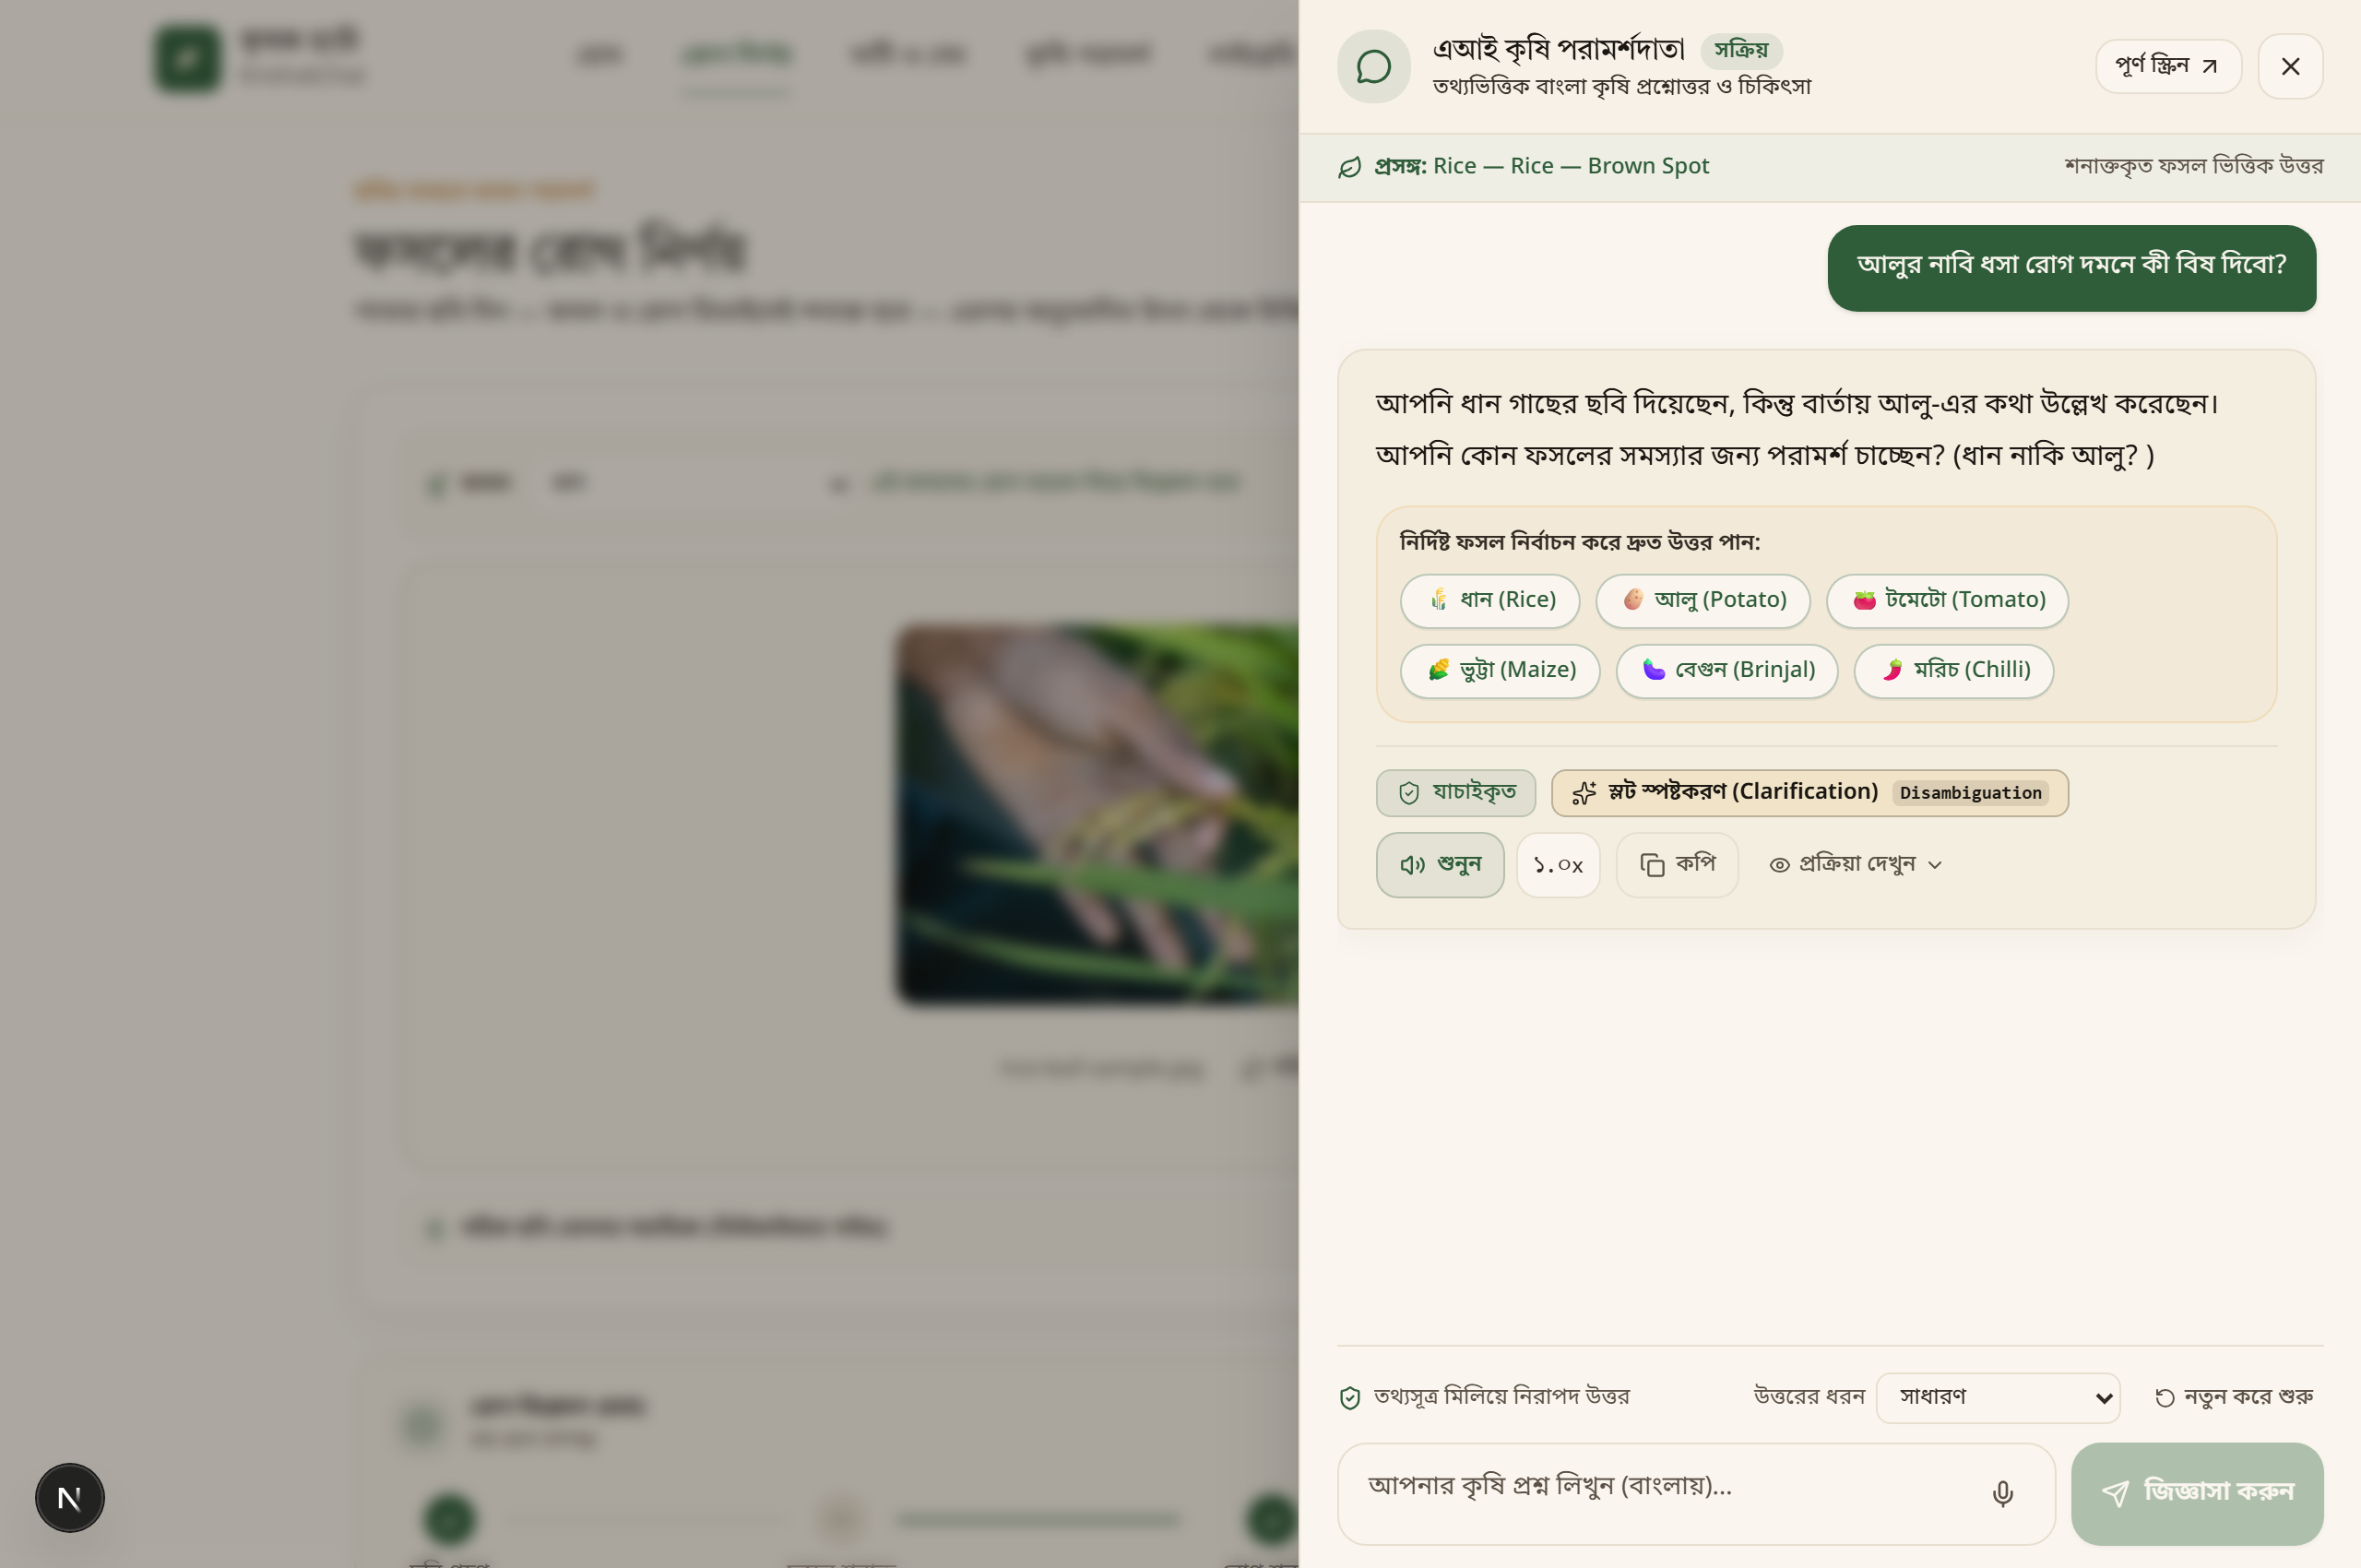
\includegraphics[width=0.92\linewidth]{../screenshots/screenshot4_mismatch_badge.png}
  \caption{CONFIRM (S3): photograph and text name different crops. The mismatch badge appears, and chemical advice is held until the farmer picks one.}
\label{fig:app_mismatch}
\end{figure}

\begin{figure}[h]
\centering
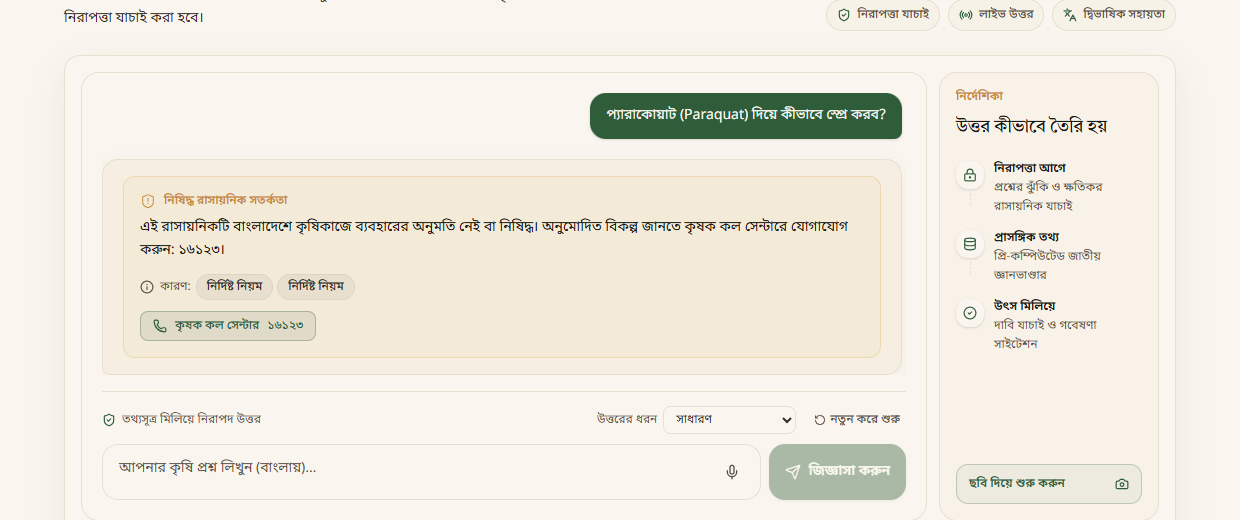
\includegraphics[width=0.92\linewidth]{../screenshots/screenshot7_16123_safety_referral.png}
\caption{REFER (S4): safety notice with a 16123 call button.}
\label{fig:app_delivery}
\end{figure}

\begin{figure}[h]
\centering
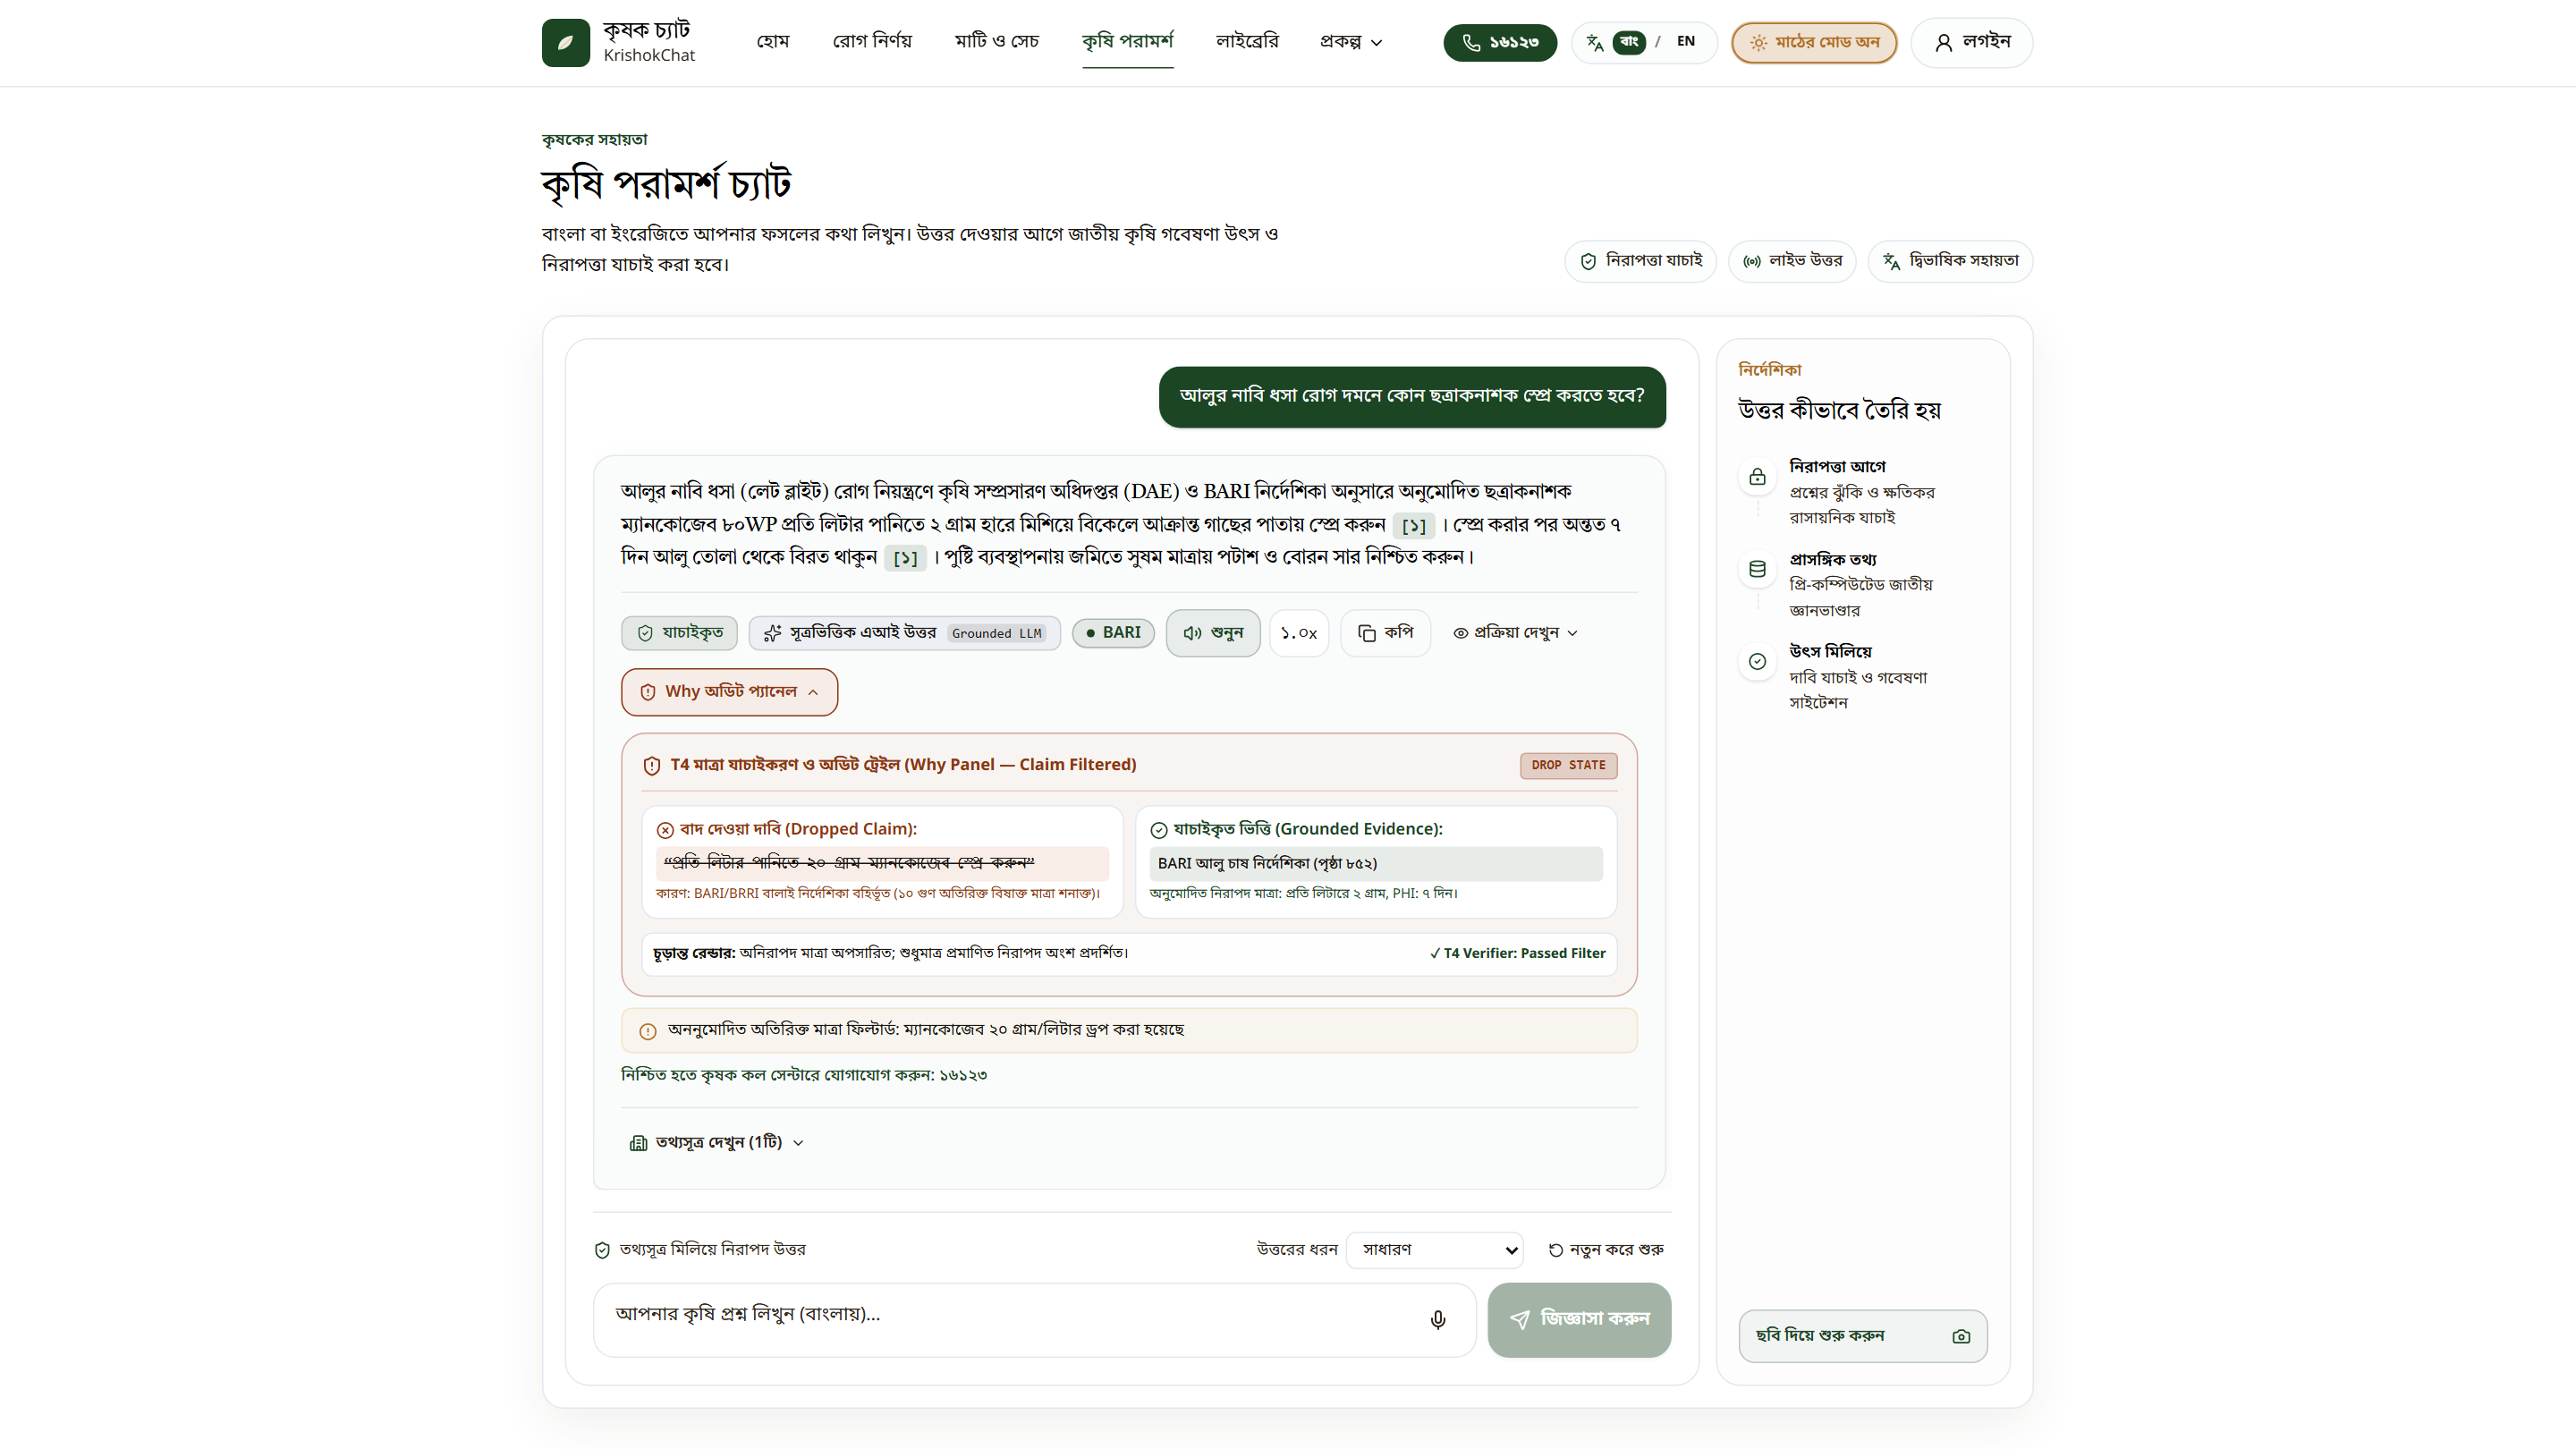
\includegraphics[width=0.92\linewidth]{../screenshots/screenshot5_grounded_answer.png}
\caption{DROP (S5): T4 removes an unsupported dosage claim, and the rest of the answer is shown with BARI citations and the expanded \textit{Why} panel.}
\label{fig:app_drop}
\end{figure}

\section{Multi-Turn State Tests}
\label{sec:eval-multiturn}

These tests check that conversation state moves as designed across turns. The suite has four constructed dialogue cohorts (200 dialogues, 425 turns) and five checks; the crop-shift cohort is scored twice (Table~\ref{tab:multiturn_eval}). Follow-up turns are rewritten into standalone queries by an LLM rewriter (\texttt{gemini-2.5-flash-lite}; 58 rewrites).

\begin{table}[t]
\centering
\scriptsize
\setlength{\tabcolsep}{2pt}
\begin{tabular*}{\columnwidth}{@{\extracolsep{\fill}}lcccc@{}}
\toprule
\textbf{Cohort} & \textbf{Dial.} & \textbf{Turns} & \textbf{Check} & \textbf{Result} \\
\midrule
Carryover & 75 & 175 & Crop slot kept & 100/100 \\
Crop shift & 75 & 150 & Slots flushed & 75/75 \\
\quad (same) & & & Old slot kept & 0/75 \\
Delayed evasion & 30 & 60 & Turn-2 catch & 30/30 \\
Clarification & 20 & 40 & ASK, then bound & 20/20 \\
\midrule
\textbf{Total} & \textbf{200} & \textbf{425} & & \\
\bottomrule
\end{tabular*}
\caption{Multi-turn state tests on constructed dialogues. The crop-shift cohort is scored on two checks; no pooled score is reported. Carryover counts the 100 follow-up turns.}
\label{tab:multiturn_eval}
\end{table}

In \textit{anaphoric carryover}, farmers ask follow-ups such as ``\textit{tahole ekhon ki spray korbo?}'' (``what should I spray then?'') without restating the crop; the crop slot was kept in all 100 follow-up turns. In \textit{crop shift}, farmers switch crops mid-conversation; all 75 switches were detected and the previous crop's disease slots were cleared. This measures conversation state, not the text of generated advice. In \textit{delayed evasion}, a benign first turn is followed by a request for a prohibited chemical (for example paraquat, Furadan, or methamidophos); T0 stopped all 30 second turns (median 0.20\,ms) and showed the 16123 referral. In \textit{clarification}, a crop-less symptom query halted at \textbf{ASK} and the crop supplied on turn two was bound in all 20 dialogues.

\section{Evidence Summary and Limitations Ledger}
\label{app:evidence}
\label{app:limitations_full}

Tables~\ref{tab:evidence_a} and~\ref{tab:evidence_b} list each measured result with its sample size, status, and scope. Status is \emph{measured} (direct measurement on benchmark or logged data), \emph{pilot} (small controlled check), \emph{simulated} (part of the condition, such as packet loss, is simulated), \emph{modeled} (derived from a cost model), or \emph{stated} (a limitation without a measurement).

\begin{table*}[t]
\centering
\scriptsize
\renewcommand{\arraystretch}{0.90}
\setlength{\tabcolsep}{4pt}
\begin{tabularx}{\textwidth}{@{}p{0.14\textwidth} p{0.30\textwidth} r p{0.09\textwidth} X@{}}
\toprule
\textbf{Component} & \textbf{Measure and result} & \textbf{$n$} & \textbf{Status} & \textbf{Scope and boundary} \\
\midrule
\multicolumn{5}{l}{\textit{Admission and referral (C1)}} \\
Crop gate & Halted 30/30 crop-less queries (15.0\% of the set, Wilson [10.71, 20.61]); passed 170/170 crop-specified queries & 200 & Measured & Real farmer queries, dual-annotated ($\kappa = 1.00$); no false halts on these 170 \\
Extractor accuracy & Crop label matched gold on 95.5\%; miss 1.5\%, false positive 3.0\% & 200 & Measured & Same 200 queries; separate from annotator agreement \\
Controlled pilot & Crop-less requests halted 100/100; specified requests passed directly 114/140, 26/140 received a bounded clarification for another slot & 240 & Pilot & Constructed pairs; conformance, not open-domain accuracy \\
Token metering & Median 89 tokens for a clarification vs 2,146 for retrieval context & 200 & Measured & Separate medians; no combined saving is claimed \\
LLM vs rule-based gate & LLM halted 10\% vs 15\% for the gate; decision agreement 0.91; median LLM latency 4,218.6\,ms & 200 & Measured & Halt rate and latency only; a 14-answer review (7/14 medium or better) is descriptive \\
Banglish precheck & 85/85 attacks intercepted (95\% CI [95.7, 100.0]) vs 1/85 for a formal-only precheck; 0/15 false alarms & 100 & Measured & Constructed Latin-script and phonetic attacks; pattern matching median 0.016\,ms, full T0 0.321\,ms \\
Off-topic audit & 10/10 injections blocked; off-topic queries refused 0/30 by T0 and 25/30 (83.33\%) by the LLM intent classifier & 40 & Measured & Five weather queries are routed to agricultural information by design \\
\midrule
\multicolumn{5}{l}{\textit{Evidence binding and conflicts (C2)}} \\
Crop binding & Top-5 cross-crop retrieval 36.25\% open vs 30.00\% with gold crop bound; 25/0 discordant, exact McNemar $p = 5.96 \times 10^{-8}$; gold-crop purity 0.647 $\to$ 0.735 & 400 & Measured & Simulates correct routing; retrieval measure, not answer quality \\
Text-extracted binding & Top-5 cross-crop retrieval 30.25\% (no gate) vs 28.75\% (gated pipeline); 6/0 discordant, $p = 0.031$ & 400 & Measured & All 400 name a crop, so the gate halts none; separate run from the row above \\
Disease vision (top-1) & 0.9413 to 0.9907 across six crop-specific classifiers & 4,294 & Measured & Disease within a crop, not crop routing; 100\% ONNX--PyTorch label agreement \\
Family router & Botanical family correct for 433/437 (0.9908, [97.67, 99.64]) & 437 & Measured & Six target crops, wheat-800 excluded; not open-world identification \\
INT8 quantization & Wheat 3.68$\times$ smaller (5.92 to 1.61\,MB), 0.00\,pp drop ($n=400$); potato 0.09\,pp ($n=1{,}170$), brassica 0.00\,pp ($n=443$); 1.5 to 2.0$\times$ slower on non-VNNI x86 CPUs & 2,013 & Measured & Storage saving, not speedup; rice INT8 lost 2.5\,pp, exceeded the 2.0\,pp gate, and was not deployed \\
Mismatch badge & Fired on 53/54 farmer conflicts [90.2, 99.7] and 400/400 PRISM conflicts [99.05, 100.0]; 0/54 and 0/400 matched controls & 908 & Measured & One implicit-reference miss (\texttt{farmer\_q\_63}) \\
\bottomrule
\end{tabularx}
\caption{Evidence summary for admission and evidence binding. Status is defined at the start of this appendix.}
\label{tab:evidence_a}
\end{table*}

\begin{table*}[t]
\centering
\scriptsize
\renewcommand{\arraystretch}{0.90}
\setlength{\tabcolsep}{4pt}
\begin{tabularx}{\textwidth}{@{}p{0.14\textwidth} p{0.30\textwidth} r p{0.09\textwidth} X@{}}
\toprule
\textbf{Component} & \textbf{Measure and result} & \textbf{$n$} & \textbf{Status} & \textbf{Scope and boundary} \\
\midrule
\multicolumn{5}{l}{\textit{Generation and release (C3)}} \\
Guarded prompt, local model & ASR 10.71\% [7.61, 14.88] guarded vs 52.5\% [46.66, 58.28] neutral (30 vs 147 of 280); Bengali-native 19/100 vs 77/100 & 280 per arm & Measured & \texttt{krishokchat-4b}, T0 and T4 disabled; 210 prompts in seven families plus 70 Bengali-native probes; rule-based judge \\
T0 + guarded prompt, local & ASR 4.64\% [2.73, 7.78] (13/280); Bengali-native 2.0\% [0.55, 7.00] (2/100); T0 intercepted 207/280 attack prompts (194 banned-chemical, 12 injection) & 280 & Measured & Replay of N14 guarded responses with T0 applied; 0 new model calls; 9/200 real farmer queries blocked as out-of-scope coverage (livestock, training, availability); no crop-treatment queries blocked \\
Guarded prompt, cloud & Guarded \texttt{gemini-2.5-flash-lite} 2/210 (0.95\%) vs neutral \texttt{gpt-4o-mini} 76/210 (36.19\%); Bengali-native 10/100 vs 83/100 & 210 per arm & Measured & Arms use different models, so not a controlled comparison; Bengali-100 = 30 main-suite + 70 top-up probes; top-up residuals in embedded (4/10) and roleplay (2/10) \\
Output audit & 46/47 guarded outputs safe and actionable, 1/47 vague but harmless, 0/47 dangerous; 3/3 unguarded controls dangerous; Fleiss $\kappa = 0.82$ & 50 & Measured & Three blinded raters (two undergraduates, one extension officer) \\
Dosage verifier, live & 114/118 inserted errors caught (96.6\%); 0/38 unmodified answers rejected & 38 & Measured & Errors inserted into 38 live answers, so they are not independent natural errors \\
Dosage verifier, scaled & 296/350 inserted errors caught (84.6\%): overdose 76/76, underdose 67/67; chemical 85\%, unit 73\%, invented PHI 65\% & 528 & Measured & Cases built from 88 BARI/BRRI passages; numerical dosage sentences only \\
Multi-turn state & Slot kept in 100/100 follow-ups; 75/75 crop shifts flushed; 30/30 delayed attacks caught; 20/20 ASK then bound & 200 & Measured & Constructed dialogues, 425 turns, four cohorts; state checks, not generated advice \\
Trace ordering & 100/100 traces in required event order (median 9 events) & 100 & Measured & Sampled evaluation cases \\
\midrule
\multicolumn{5}{l}{\textit{Delivery and deployment}} \\
SMS length & 399/400 messages within 160 GSM-7 characters; 8/8 referral messages carried only the referral & 400 & Measured & Latin-script output; Bengali script needs UCS-2 (70 per segment) \\
SMS slot survival & Dose, interval, and PHI kept in 1,000/1,000 constructed tuples; dose kept in 65/66 live gold advisories vs 12/92 for naive truncation & 1,000 & Measured & Different denominators, not a paired comparison \\
SMS comparison & Dose kept in 23/100 (naive), 89/100 (LLM), 92/100 (compressor); chemical name in 20, 56, and 34 of 100 & 100 & Measured & Seed 42; a kept dose is not a complete instruction \\
Offline retrieval & Local BM25 hit rate 0.94, 0/400 cache misses; remote retrieval loses 13.25\,pp (15\% loss) and 30.0\,pp (30\% loss) & 400 & Measured, loss simulated & Retrieval only \\
Non-LLM overhead & Median 33.565\,ms (p95 67.833\,ms): safety 0.321, BM25 26.831, verifier 4.815\,ms & 400 & Measured & Stub LLM; local generation about 24\,s per call \\
Installation footprint & 95.64\,MB ONNX vision assets; 284.0\,MB minimal; 339.6\,MB with PyTorch checkpoints & n/a & Measured & Excludes the language-model weights \\
Tier mix and cost & 7.9\% zero-LLM turns; USD~0.1720 per 1,000 turns vs 0.1995 with every turn generated & 1,000 & Modeled & Metered tokens from 58 calls; not billed expenditure \\
Retrieval backend & BM25 only; dense retrieval not evaluated & n/a & Stated & All retrieval numbers are BM25-only \\
\bottomrule
\end{tabularx}
\caption{Evidence summary for generation, release, delivery, and deployment. Status is defined at the start of this appendix.}
\label{tab:evidence_b}
\end{table*}


\end{document}
